\pdfoutput=1
\documentclass[11pt]{amsart}
\usepackage{amsmath,amssymb,amsthm,mathtools,mathrsfs}
\usepackage[margin=1.2in]{geometry}
\usepackage{graphicx,booktabs,adjustbox,tikz}
\usetikzlibrary{arrows.meta,positioning,calc}
\usepackage{xcolor,placeins}
\usepackage[colorlinks=true,linkcolor=blue,citecolor=blue,urlcolor=blue]{hyperref}
\hypersetup{pdfauthor={Bernd Johannes Wuebben},pdftitle={Hermitian--Einstein metrics and small spectra for three-step extensions}}
\setlength{\emergencystretch}{2em}
\newtheorem{theorem}{Theorem}[section]
\newtheorem{proposition}[theorem]{Proposition}
\newtheorem{lemma}[theorem]{Lemma}
\newtheorem{corollary}[theorem]{Corollary}
\theoremstyle{definition}
\newtheorem{definition}[theorem]{Definition}
\newtheorem{example}[theorem]{Example}
\newtheorem{question}[theorem]{Question}
\theoremstyle{remark}
\newtheorem{remark}[theorem]{Remark}
\newcommand{\CC}{\mathbb C}
\newcommand{\RR}{\mathbb R}
\newcommand{\ZZ}{\mathbb Z}
\newcommand{\PP}{\mathbb P}
\newcommand{\cO}{\mathcal O}
\newcommand{\cI}{\mathcal I}
\newcommand{\db}{\bar\partial}
\newcommand{\tr}{\operatorname{tr}}
\newcommand{\rk}{\operatorname{rk}}
\newcommand{\Hom}{\operatorname{Hom}}
\newcommand{\Coh}{\operatorname{Coh}}
\newcommand{\Vol}{\operatorname{Vol}}
\newcommand{\HYM}{\operatorname{HYM}}
\newcommand{\YM}{\operatorname{YM}}
\newcommand{\Gr}{\operatorname{Gr}}
\newcommand{\id}{\operatorname{id}}
\title[Metrics and small spectra for three-step extensions]{Hermitian--Einstein metrics and small spectra\\for three-step extensions}
\author{Bernd Johannes Wuebben}
\subjclass[2020]{53C07 (primary); 32Q15, 14D20, 58J50 (secondary)}
\keywords{Hermitian--Einstein metric, stability wall, three-step extension,
Dolbeault spectrum, quiver relation, metric response}
\date{October 31, 2026\\This version: October 31, 2026}

\newcommand{\End}{\operatorname{End}}
\newcommand{\diag}{\operatorname{diag}}
\newcommand{\ad}{\operatorname{ad}}
\newcommand{\HH}{\mathsf H}
\newcommand{\cK}{\mathcal K}
\newcommand{\cR}{\mathcal R}
\newcommand{\cF}{\mathcal F}
\newcommand{\cD}{\mathscr D}

\begin{document}
\begin{abstract}
We prove uniform relative asymptotics for every small Dolbeault
eigenvalue on trace-free endomorphism-valued zero-forms in a class of
three-step Hermitian--Einstein extensions, allowing arbitrary separation
of positive spectral scales. The graded factors are distinct line bundles
of equal slope at a reference polarization on a compact K\"ahler manifold.
Adjacent extension classes vary in fixed cohomology subspaces; the
remaining terms are quadratic coexact Hodge primitives of their
compositions, with no independent first-to-third-layer parameters.
Assume integrability and a connected extension graph. At nearby
polarizations, suppose diagonal rescaling balances the squared norms
of the adjacent classes against the slope differences, with sufficiently
small sum of rescaled squared norms. The rescaled split metric then
approximates the Hermitian--Einstein metric with the same determinant,
with logarithmic error bounded by a uniform constant times that sum.
Every small eigenvalue has the same relative accuracy with respect to
the corresponding eigenvalue of the graph Laplacian weighted by these
squared norms;
the complementary spectrum has a uniform positive gap. The proof
controls curvature traces by the energy crossing each vertex cut.
A family on the product of three projective lines has a spectral scale
undetected by its polarization parameters. At each fixed bundle in
this family, both singular values of the intrinsic metric response to
the two polarization parameters agree, with the same relative accuracy,
with those of the differentiated finite balancing equation.
\end{abstract}

\maketitle


% Source: sections/01_introduction.tex
\section{Introduction}\label{sec:introduction}

Near a stability wall, a Hermitian--Einstein connection approaches the
connection on its graded object. The small endomorphism eigenvalues record
how the graded factors remain joined. When some extension directions are
much weaker than others, convergence of the connection does not by itself
determine each small eigenvalue: an error small compared with the total
extension energy may exceed the weakest eigenvalue. The same difficulty
appears when one asks how the Hermitian--Einstein metric responds to a
change of polarization.

For extensions of two polystable bundles, a finite weighted graph can
retain every small spectral scale. We consider the next case, where
extension arrows compose. Their compositions can be nonzero differential
forms, and their cohomology classes can impose genuine relations on the
extension parameters. The nonlinear terms required by integrability must
be included in both the metric construction and the spectral comparison.
We prove relative estimates for a specified three-step class, uniformly
in its extension directions and in all positive scale ratios.

\subsection{A first example and the general statement}
The simplest example is a fixed rank-three bundle on $(\PP^1)^3$ with
graded lines
\[
 \cO(-1,-1,2),\qquad \cO(1,-2,1),\qquad \cO.
\]
Two nonzero adjacent harmonic extensions have a nonzero but exact
composition form. A quadratic endpoint term makes their matrix
integrable. In two actual polarization coordinates $k_1,k_2>0$, the
finite model is the path with edge weights $k_1,k_2$, whose positive
eigenvalues are
\[
 \nu_{1,2}=k_1+k_2\mp\sqrt{k_1^2-k_1k_2+k_2^2}.
\]
Section~\ref{sec:chain} constructs the bundle, proves that it intrinsically
requires three polystable layers at the reference slope, and specifies
its balanced metric independently of the unknown HE metric. The actual
small eigenvalues satisfy $\lambda_j/\nu_j=1+O(k_1+k_2)$, and the rest
of the spectrum stays separated from zero. This remains true if one
parameter is exponentially smaller than the other.

The general construction starts with distinct equal-slope line factors
$F_i$, divided into three ordered layers. For each pair in adjacent layers
choose a finite-dimensional space of harmonic extension classes. The
endpoint correction is the negative coexact Green primitive of the sum
of their two-arrow products. There are no independent linear endpoint
parameters. Hodge decomposition makes integrability exactly equivalent
to the vanishing of the cup-product obstruction. We call this the
canonical three-step family; its complete definition is in
Section~\ref{sec:canonical}.

For each nonzero adjacent block draw an edge from source to target. Write
$n_e$ for its initial weight, the squared harmonic norm divided by the base volume.
Let $D$ be the incidence matrix, with column $e_i-e_j$ for $j\to i$,
and let $b_i=\kappa_E-\kappa_i$ be the centered HE constants of the
factors. A positive diagonal gauge is chosen by the finite equation
\[
 Dw=b,\qquad w_e=n_e e^{x_i-x_j},\qquad \sum_i x_i=0.
\]
If the support is connected and admits a positive flow, this gauge exists
uniquely. Put $\sigma=\sum_e w_e$ and let
$h_{\mathrm{bal}}=g_0^*h_0$, where $g_0=\diag(e^{x_i/2})$.
Let $\nu_1\le\cdots\le\nu_{m-1}$ be the graph eigenvalues on
trace-free diagonal constants with unit vertex masses.

Theorem~\ref{thm:uniform} constructs the fixed-determinant HE metric and
proves
\begin{equation}\label{eq:intro-comparison}
 e^{-C\sigma}h_{\mathrm{bal}}\le H\le e^{C\sigma}h_{\mathrm{bal}},
 \qquad
 \left|\frac{\lambda_j}{\nu_j}-1\right|\le C\sigma,
 \qquad \lambda_m\ge\gamma>0.
\end{equation}
Here $\lambda_j$ are the actual Dolbeault eigenvalues on complex
trace-free endomorphism-valued zero-forms, counted with complex
multiplicity. The constants depend only on the fixed coefficient spaces
and a compact neighborhood of background metrics. There is no restriction
on positive edge ratios, on eigenvalue ratios, or on the rank of the
obstruction derivative. The positive-flow condition is also exactly the
local stability criterion for this family. At disconnected small
coefficients a separate auxiliary statement identifies the kernel as the
diagonal constants on each graph component.

\subsection{Why the estimates remain relative}
After solving the elliptic equation complementary to constant diagonal
endomorphisms, the remaining curvature has the form
\[
 \mathcal F=-b+\mu+R.
\]
Harmonicity removes the first-order terms, and the three-layer sign
symmetry removes the cubic jet. A total estimate $R=O(\sigma^2)$
follows, but is too weak for \eqref{eq:intro-comparison}. The useful
estimate is instead
\begin{equation}\label{eq:intro-cut}
 \left|\sum_{i\in S}R_i\right|
 \le Cq\sum_{e\text{ crossing }S}n_e
 \qquad\text{for every vertex cut }S,
\end{equation}
where $q$ is the current total linear-arrow energy.
Removing all independent coefficients crossing a cut also removes every
quadratic path with separated endpoints. The resulting unitary connection
splits, and its integrated partial curvature trace is fixed by Chern--Weil.
This remains valid even when the cut leaves the obstruction locus.
The resulting exact vanishing and cut-sign symmetry imply
\eqref{eq:intro-cut} by Taylor expansion.

A finite degree argument now corrects the balanced gauge by $O(\sigma)$.
On a boundary sphere, sort its diagonal values and select a cut across a
largest adjacent gap. The finite moment increment across that cut is
positive and dominates the residual by the same cut energy. That energy
may be arbitrarily small, but it appears on both sides. There is no need
to divide an absolute remainder by a weak eigenvalue.

For the spectrum, each quadratic endpoint commutator is estimated along
the two edges of its path. Its energy is at most $Cq$ times the linear
graph energy, separately for every diagonal direction. Co-closedness
removes the first coupling to the complementary elliptic space, whose
spectral gap is fixed. Min--max then gives every relative eigenvalue
estimate, including repeated eigenvalues. Sections~\ref{sec:correction}
and \ref{sec:spectrum} provide the full arguments.

\subsection{A geometric family and metric response}
The four lines
\[
 \cO(-2,-2,4),\quad\cO(1,-2,1),\quad\cO(-2,1,1),\quad\cO
\]
on $(\PP^1)^3$ give a nonlinear diamond with $24$ adjacent-layer
coordinates and five quadratic relations. Its endpoint primitive is
nonzero. Section~\ref{sec:diamond} proves that full-support torus orbits
are exactly bundle isomorphism classes over the fixed base and constructs
a local $16$-dimensional family of nonisomorphic bundles. The theorem is
uniform on that family, at points where the obstruction derivative loses
rank, and on every connected support satisfying its own stable inequalities.

The finite weights depend on an orbit invariant
$\rho=n_{12}n_{24}/(n_{13}n_{34})$ in addition to the polarization.
An explicit family has $\rho=1+|M|^2$. Even with the two polarization
parameters constrained by $k=3l/5$, its smallest eigenvalue divided by
the total energy tends to zero as $|M|\to\infty$. Thus a uniform
spectral description must retain extension-orbit data.

We also determine how the actual HE metric changes with these two
polarization parameters while the bundle is fixed. Its intrinsic tangent
is $(H^{-1}\partial_vH)_0$, measured in the current normalized $L^2$
norm. The finite prediction is the derivative of the balancing equation,
\[
 \mathcal R_0=L(w)^{-1}\bigl(B_0-D\diag(w)A_s\bigr),
\]
where $B_0$ differentiates the centered demands and $A_s$ differentiates
the logarithmic harmonic norms. Both matrices are printed in
Section~\ref{sec:finite-response}. Theorem~\ref{thm:response} compares
the two singular values of this operator with the two singular values of
the actual metric response, each to relative error $O(\sigma)$.

A metric inequality cannot simply be differentiated to prove this result.
We differentiate the cut estimates, obtain a directional inverse bound,
and retain the exact intrinsic metric velocity and the changing
fixed-bundle identification. The unbounded family then has two actual
response scales $1/\delta$ and $1/l$, where
$\delta/l\sim\sqrt{3/(5\rho)}$. Section~\ref{sec:response-scales}
computes their leading constants and the two polarization directions that
distinguish them. The third graph eigenvalue does not create a third
singular value for a two-dimensional input.

\subsection{Relation to earlier work}
Clarke--Tipler prove local chamber and HYM convergence results for a fixed
semistable bundle with abelian graded automorphisms, and construct the
complementary reduction on an ambient coefficient ball
\cite[Proposition~1.1, Theorem~1.2 and Propositions~3.1--3.2]{clarketipler2024}.
Their setting already includes successive extensions. Their Remark~1.4
distinguishes compact families from the problem of uniformity over all
small graded deformations. Delloque develops complementary reduction and
quantitative convergence under metric variation with a broader graded
automorphism group \cite[Propositions~4.2,4.7 and Theorems~4.8--4.9]{delloque2025}.
The present result concerns the stated canonical three-step family. Its
additional conclusions are relative control of every small eigenvalue
and the explicit metric response, uniform through unrestricted positive
scale separation and variation of the adjacent extension directions.

The cut-relative correction and energy-relative spectral argument have
two-step predecessors in \cite{wuebben2026bipartite,wuebben2026repeated}.
The intrinsic differentiation and complementary inverse were used for
two-step response in \cite{wuebben2026response}. We retain these mechanisms
and prove the new nonlinear geometric and differentiated cut estimates
needed here. The scalar distinct-line theorem does not subsume the
matrix multiplicities in \cite{wuebben2026repeated}. Nor does the
$24$-coordinate diamond exhaust the full graded deformation space.
Quotient metrics, stabilizer-changing derivatives and actual flow require
separate arguments.

% Source: sections/02_examples.tex
\section{A chain and a first obstructed example}\label{sec:chain}

We begin with a fixed rank-three bundle whose two small eigenvalues have
closed formulas. It displays the nonlinear term needed for integrability
without an obstruction equation on its parameters. A tensor-product diamond
then separates those two issues: its integrability equation is nontrivial,
but it needs no quadratic primitive. Section~\ref{sec:diamond} will combine
both phenomena on a family of genuinely different bundles.

\begin{figure}[htbp]
\centering
\begin{adjustbox}{max width=\textwidth,center}
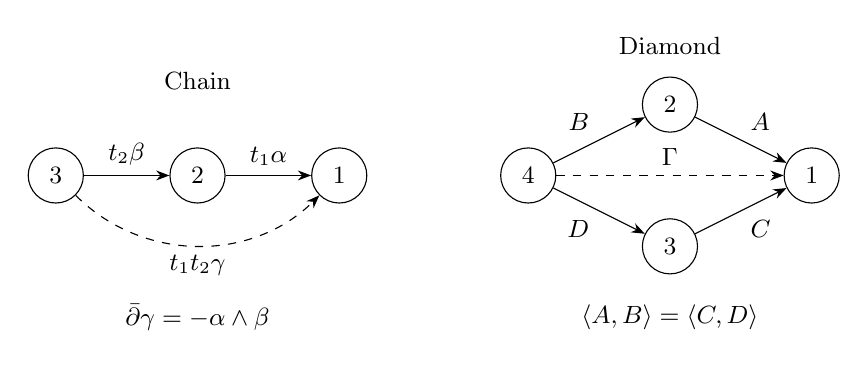
\begin{tikzpicture}[>=Stealth,vertex/.style={circle,draw,minimum size=7mm,inner sep=0pt},every node/.style={font=\small}]
\node[vertex] (c3) at (0,0) {$3$};
\node[vertex] (c2) at (1.8,0) {$2$};
\node[vertex] (c1) at (3.6,0) {$1$};
\draw[->] (c3) -- node[above] {$t_2\beta$} (c2);
\draw[->] (c2) -- node[above] {$t_1\alpha$} (c1);
\draw[->,dashed] (c3) to[bend right=45] node[below] {$t_1t_2\gamma$} (c1);
\node at (1.8,1.2) {Chain};
\node[align=center] at (1.8,-1.8) {$\bar\partial\gamma=-\alpha\wedge\beta$};
\node[vertex] (d4) at (6,0) {$4$};
\node[vertex] (d2) at (7.8,0.9) {$2$};
\node[vertex] (d3) at (7.8,-0.9) {$3$};
\node[vertex] (d1) at (9.6,0) {$1$};
\draw[->] (d4) -- node[above left] {$B$} (d2);
\draw[->] (d2) -- node[above right] {$A$} (d1);
\draw[->] (d4) -- node[below left] {$D$} (d3);
\draw[->] (d3) -- node[below right] {$C$} (d1);
\draw[->,dashed] (d4) -- node[above] {$\Gamma$} (d1);
\node at (7.8,1.65) {Diamond};
\node at (7.8,-1.8) {$\langle A,B\rangle=\langle C,D\rangle$};
\end{tikzpicture}
\end{adjustbox}
\caption{Two three-step constructions. Solid arrows are the independent
harmonic extension classes; dashed arrows are the quadratic corrections
required by integrability. The chain of Section~\ref{sec:chain} has an
exact composition and no parameter relation. The nonlinear diamond of
Section~\ref{sec:diamond} has both a nonzero correction and a cup-product
relation. The graph for the leading spectral model contains only the
solid edges.}
\label{fig:extension-graphs}
\end{figure}


\subsection{A chain on three projective lines}
On $X=(\PP^1)^3$, normalize the Fubini--Study forms by
$\int_{\PP^1}\omega_i=1$. Give all product line bundles their fixed
product metrics, with $iF_{\cO(d)}=2\pi\sum_i d_i\omega_i$. Set
\[
 F_1=\cO(-1,-1,2),\qquad F_2=\cO(1,-2,1),\qquad F_3=\cO.
\]
The three lines have slope zero at $\omega_1+\omega_2+\omega_3$.
Their selected adjacent Hom bundles and endpoint bundle are
\[
 A=\cO(-2,1,1),\qquad B=\cO(1,-2,1),\qquad C=\cO(-1,-1,2).
\]
Projective-line cohomology and K\"unneth give
\[
 h^1(A)=h^1(B)=4,\qquad H^q(C)=0\quad\text{for every }q.
\]
Every off-diagonal Hom has zero $H^0$, because its degree vector has a
negative entry. We use the standard formulas recorded in
\cite[Tags~01XT and 0BED]{stacks}.

Choose nonzero harmonic $\cO(-2)$-valued $(0,1)$-forms $\eta_1,\eta_2$
on the first two factors and nonzero holomorphic sections $s_i$ of
$\cO(1)$, with another such section $s'_3$ on the third. Put
\[
 \alpha=\eta_1\otimes s_2\otimes s_3,\qquad
 \beta=s_1\otimes\eta_2\otimes s'_3.
\]
They remain harmonic for $\omega_h=\sum_i h_i\omega_i$: the product
Laplacian is the sum of factor Laplacians multiplied by $h_i^{-1}$.
Their composition is a nonzero differential form. On the product of open
sets where the factors are nonzero, its two differential legs are independent.
Its cohomology class vanishes because $H^2(C)=0$.

Let $D_C$ be the Dolbeault operator on $C$, and let $G_{2,h}$ be
its Green operator on $(0,2)$-forms, zero on harmonic forms. Put
\begin{equation}\label{eq:chain-primitive}
 \gamma_h=-D_{C,h}^*G_{2,h}(\alpha\wedge\beta),\qquad
 D_C\gamma_h=-\alpha\wedge\beta,\quad D_{C,h}^*\gamma_h=0.
\end{equation}
In particular $\gamma_h\ne0$. Write $D_0$ for the split Dolbeault
operator on $F_1\oplus F_2\oplus F_3$. The family
\begin{equation}\label{eq:chain-matrix}
 N_h(t)=\begin{pmatrix}
 0&t_1\alpha&t_1t_2\gamma_h\\
 0&0&t_2\beta\\0&0&0
 \end{pmatrix},\qquad \bar\partial_{h,t}=D_0+N_h(t)
\end{equation}
is integrable for every $(t_1,t_2)\in\CC^2$. Equation~\eqref{eq:chain-primitive}
cancels its sole possible $(0,2)$ curvature entry. It is also co-closed.
The parameter space selects one direction in each adjacent $H^1$; it is
not the full graded deformation space. For example the reverse group
$H^1(\Hom(F_1,F_3))$ has dimension four.

Under a diagonal gauge, $t_1,t_2$ acquire ratios $g_1/g_2,g_2/g_3$;
their product has exactly the endpoint ratio $g_1/g_3$. Thus every
nonzero pair gives the same holomorphic isomorphism class for fixed $h$.
The bundle can also be held fixed as $h$ varies. The form
$\gamma_h-\gamma_1$ is closed and $H^1(C)=0$, so choose smoothly
$f_h$ with $D_Cf_h=\gamma_h-\gamma_1$, for example by the reference
Green inverse. With convention $D'=gDg^{-1}$, the gauge
\[
 \Phi_h=I-f_hE_{13}
\]
sends the unit-parameter reference bundle $E$ to its $h$-presentation.
Conjugation contributes $+D_Cf_h$ in that entry; every other product with
this endpoint matrix vanishes. The gauge has determinant one.

\subsection{Why three layers are intrinsic}
Let $E_{12}$ be the nonsplit $\alpha$ extension of $F_2$ by $F_1$.
The class $\beta$ lifts uniquely to an extension of $F_3$ by $E_{12}$:
$H^2(C)=0$ gives existence, and $H^1(C)=0$ gives uniqueness. Its image
$\beta$ is nonzero. This gives
$0\subset F_1\subset E_{12}\subset E$, agreeing with
\eqref{eq:chain-matrix}.

At the reference polarization the bundle is semistable. The connecting
maps of these sequences and the off-diagonal Hom vanishings imply
\[
 \Hom(F_1,E)=\CC,\qquad \Hom(F_2,E)=\Hom(F_3,E)=0.
\]
For instance the connecting map for $F_2$ sends its identity to the
nonzero class $\alpha$, and the connecting map for $F_3$ has nonzero
image $\beta$.

A stable locally free bundle of slope zero mapping to $E$ maps, after
factoring through earlier terms, nontrivially to one line quotient.
A stable source of rank greater than one cannot have a rank-one quotient
of nonpositive slope. A nonzero map between equal-slope lines has no zero
divisor and is an isomorphism. Thus every stable summand of a slope-zero
polystable subbundle must be one of the $F_i$. The displayed Hom groups
force its image to be the single copy of $F_1$. But $E/F_1$ is the
nonsplit $\beta$ extension and is not polystable. Therefore $E$ cannot
be expressed as an extension of two polystable bundles of the reference
slope. The third layer is not an artifact of the chosen matrix.

\subsection{The two eigenvalues}
Fix $h_3=1$ and set
\[
 h_1=(1+k_1/(2\pi))^{-1},\qquad
 h_2=(1+k_2/(2\pi))^{-1}.
\]
For small signed $k_i$ these are genuine K\"ahler forms. Since
$\kappa_{\cO(d)}=2\pi\sum_i d_i/h_i$, the centered demands are
\[
 b=(k_1,k_2-k_1,-k_2).
\]
Let $c_1(h)=\|\alpha\|_2^2=c_1(1)/h_1$ and
$c_2(h)=\|\beta\|_2^2=c_2(1)/h_2$, with volume-normalized norms.
For $k_1,k_2>0$ the independently balanced amplitudes are
$t_i^0=\sqrt{k_i/c_i(h)}$. The positive determinant-one gauge is
\[
 g(t)=\diag\bigl(t_1^{2/3}t_2^{1/3},\,
 t_1^{-1/3}t_2^{1/3},\,t_1^{-1/3}t_2^{-2/3}\bigr).
\]
Define $h_{\mathrm{bal}}=(g(t^0)\Phi_h)^*h_0$ on the fixed $E$.
Its finite operator is
\begin{equation}\label{eq:chain-laplacian}
 L(k)=\begin{pmatrix}
 k_1&-k_1&0\\-k_1&k_1+k_2&-k_2\\0&-k_2&k_2
 \end{pmatrix}.
\end{equation}
Its characteristic polynomial is
$\lambda(\lambda^2-2(k_1+k_2)\lambda+3k_1k_2)$. Thus, putting
$\sigma=k_1+k_2$, its two positive eigenvalues are
\begin{equation}\label{eq:chain-eigenvalues}
 \nu_{1,2}=\sigma\mp\sqrt{k_1^2-k_1k_2+k_2^2}.
\end{equation}
Theorem~\ref{thm:uniform} gives the actual metric estimate
\eqref{eq:main-metric}, $\lambda_j/\nu_j=1+O(\sigma)$ for $j=1,2$,
and $\lambda_3\ge\gamma$. Its hypotheses are precisely the three
singleton layers, the two chosen harmonic lines and primitive
\eqref{eq:chain-primitive}. The positive flow condition is $k_1,k_2>0$.
Necessity is also visible in the subbundles $F_1$ and $E_{12}$.
There is no restriction on $k_1/k_2$, including exponentially separated
approaches to the wall.

In this example the exact diagonal commutator energy has the additional
term
\[
 \|\gamma_h\|_2^2|t_1t_2|^2|\xi_1-\xi_3|^2.
\]
The inequality $|\xi_1-\xi_3|^2\le2|\xi_1-\xi_2|^2+
2|\xi_2-\xi_3|^2$ makes it a relative $O(\sigma)$ correction to the
path form. This elementary calculation is the model for the general
spectral proof in Section~\ref{sec:spectrum}.

\subsection{An obstruction that comes from a tensor product}\label{subsec:product}
On $(\PP^1)^4$ put $U=\cO(-1,1)$, $V=\cO(1,-1)$ on the first
two factors, and use $U',V'$ with the same degrees on the last two.
Take
\[
 (F_1,F_2,F_3,F_4)
 =(U\boxtimes U',V\boxtimes U',U\boxtimes V',V\boxtimes V').
\]
Choose nonzero harmonic forms $\alpha$ in
$H^1(\cO(-2,2,0,0))$ and $\beta$ in
$H^1(\cO(0,0,-2,2))$. Each group has dimension three. Their product is
a nonzero harmonic class in $H^2(\cO(-2,2,-2,2))$, of dimension nine;
the endpoint $H^1$ vanishes. The four blocks
\[
 N_{12}=x\alpha,\quad N_{13}=y\beta,\quad
 N_{24}=v\beta,\quad N_{34}=w\alpha
\]
satisfy
\begin{equation}\label{eq:product-obstruction}
 (D_0+N)^2=(xv-yw)\alpha\wedge\beta\,E_{14}.
\end{equation}
Thus $xv=yw$ is a genuine obstruction equation. No endpoint form can
repair a nonzero value, because its cohomology class is nonzero. The
canonical quadratic primitive is zero here: the products are already
harmonic. At unit coefficients the bundle is $E_A\boxtimes E_B$, the
tensor product of the two nonsplit rank-two extensions.

At the reference slope its maximal polystable subbundle is $F_1$.
Indeed K\"unneth gives $\Hom(F_1,E)=\CC$ and $\Hom(F_i,E)=0$ for
$i>1$; the preceding stable-source argument applies to its line filtration.
Its quotient by $F_1$ has a nonsplit extension of $F_4$ by $F_2\oplus F_3$.
It therefore also needs three polystable layers. This geometric fact does
not remove its tensor-product origin. The full graded cohomology dimensions
are $(h^0,h^1,h^2)=(4,24,36)$; the four selected scalar parameters are
only a subfamily.

Set $h_2=h_4=1$, $h_1=(1+a/(2\pi))^{-1}$ and
$h_3=(1+b/(2\pi))^{-1}$. The centered demands are
$(a+b,-a+b,a-b,-a-b)$. For $a,b>0$, choosing
$s=\sqrt{a/\|\alpha\|_2^2}$ and $t=\sqrt{b/\|\beta\|_2^2}$
gives balanced coefficients $(s,t,t,s)$ and weights $(a,b,b,a)$.
The gauge is
\[
 g_0=\diag(\sqrt{st},\sqrt{t/s},\sqrt{s/t},1/\sqrt{st}).
\]
The positive graph eigenvalues, in increasing order, are
$2\min(a,b),2\max(a,b),2(a+b)$. The total arrow energy in the
normalization of Theorem~\ref{thm:uniform} is $2(a+b)$; its error is
therefore $O(a+b)$. The theorem gives the actual HE metric and all three
relative spectral estimates, and stability holds exactly for $a,b>0$.
These conclusions can also be understood from the two factor problems.

This example makes a cut obstruction particularly visible. Removing the
crossing arrows for $S=\{1,2,4\}$ sets $y=w=0$ but leaves $xv$.
The residual in \eqref{eq:product-obstruction} is then nonzero and
nonexact. The general proof uses the auxiliary unitary connection at this
cut, retaining the topological partial trace even though integrability fails.

% Source: sections/03_canonical_family.tex
\section{Canonical three-step extensions and finite balance}\label{sec:canonical}

We now specify the class for which the comparison is uniform. The linear
extension classes join adjacent layers. Their compositions determine a
quadratic correction between the first and third layers. There are no
independent linear parameters between those endpoint layers.

\subsection{Geometric data and the obstruction}
Let $X$ be a fixed compact connected K\"ahler manifold of complex dimension
$n$. Let $F_1,\ldots,F_m$, $m\ge2$, be pairwise nonisomorphic holomorphic
line bundles of equal slope at a reference form $\omega_0$. We assume
\begin{equation}\label{eq:cross-hom}
 H^0(X,\Hom(F_j,F_i))=0\qquad(i\ne j).
\end{equation}
For distinct line bundles of equal slope this follows from stability.
Partition the indices into layers $I_0,I_1,I_2$. The allowed arrows
$j\to i$ have $j\in I_{r+1}$ and $i\in I_r$. For each such ordered
pair choose a subspace
\[
 V_{ij}\subset H^1(X,\Hom(F_j,F_i)),\qquad
 V=\bigoplus_{ij}V_{ij}.
\]
All directions with the same endpoints are included in one space $V_{ij}$.
A zero space contributes no arrow.

Let $\omega_s$ be a smooth family of K\"ahler forms in a neighborhood of
zero with compact closure in its parameter domain. Choose smoothly varying
HE metrics $h_{i,s}$ on the lines, and write $h_{0,s}$ for their orthogonal
sum. Their mean curvatures and the centered demands are
\begin{equation}\label{eq:demands}
 \kappa_i(s)=\frac{2\pi\deg_s F_i}{\Vol_s X},\qquad
 \kappa_E(s)=\frac1m\sum_i\kappa_i(s),\qquad
 b_i(s)=\kappa_E(s)-\kappa_i(s).
\end{equation}
Here $\deg_s F=\int_Xc_1(F)\wedge\omega_s^{n-1}/(n-1)!$ and
$\Vol_sX=\int_X\omega_s^n/n!$. All $L^2$ inner products in this paper
are divided by $\Vol_sX$. A constant diagonal endomorphism therefore has
squared norm $\sum_i|\xi_i|^2$.

Denote the split Dolbeault operator by $D_0$ and its Chern connection by
$\nabla_{0,s}$. Let $\HH_s(z_{ij})$ be the harmonic representative of
$z_{ij}\in V_{ij}$. The harmonic inclusions and their Gram matrices vary
smoothly with $s$, and these Gram matrices are uniformly positive on the
chosen parameter closure. The linear block form $L_s(z)$ has entries
$\HH_s(z_{ij})$. For $i\in I_0$, $k\in I_2$, define
\begin{equation}\label{eq:quadratic-primitive}
 Q_{ik,s}(z)=-D_{ik,s}^*G_{ik,2,s}
       \sum_{j\in I_1}\HH_s(z_{ij})\wedge\HH_s(z_{jk}),
 \qquad N_s(z)=L_s(z)+Q_s(z),
\end{equation}
where $D_{ik}$ acts on $\Hom(F_k,F_i)$ and $G_{ik,2,s}$ is its
Green operator on $(0,2)$-forms, zero on harmonic forms. Every other
entry of $Q_s$ is zero. The cohomological obstruction is
\begin{equation}\label{eq:obstruction}
 \Omega_{ik}(z)=\sum_j z_{ij}\smile z_{jk}
 \in H^2(X,\Hom(F_k,F_i)),\qquad Z=\Omega^{-1}(0).
\end{equation}
The cup product in this formula is independent of $s$.

\begin{lemma}\label{lem:canonical}
On the whole coefficient space $V$,
\begin{equation}\label{eq:canonical-identities}
 (D_0+N_s(z))^2=(\HH_s\Omega_{ik}(z))_{ik},\qquad
 D_{0,s}^*N_s(z)=0.
\end{equation}
Consequently $D_0+N_s(z)$ is integrable exactly when $z\in Z$.
The map $Q_s$ is quadratic with uniform bilinear bounds in every fixed
spatial norm. A constant diagonal gauge $g$ acts by $g_i/g_j$ on
$z_{ij}$ and satisfies $N_s(g\cdot z)=gN_s(z)g^{-1}$.
\end{lemma}

\begin{proof}
The wedge products in \eqref{eq:quadratic-primitive} are closed. Hodge
decomposition gives their negative, plus their harmonic projection, after
applying $D_{ik}$ to $Q_{ik,s}$. These are exactly the entries of
$D_0N_s+N_s\wedge N_s$: there is no product involving a quadratic
endpoint block because there are only three layers. Harmonicity gives
co-closedness for the linear terms, and $(D_{ik,s}^*)^2=0$ gives it for
the quadratic terms. The cohomology dimensions are fixed, so the positive
spectra on the harmonic complements stay uniformly separated from zero.
Smooth elliptic parameter dependence gives the asserted Green bounds.
Finally each product along $k\to j\to i$ has character
$(g_i/g_j)(g_j/g_k)=g_i/g_k$, proving equivariance.
\end{proof}

For $z\in Z$, write $E_{s,z}$ for this holomorphic bundle. The definition
allows singularities of $Z$ and changes in the rank of $D\Omega$. It does
not assert that $E_{s,z}$ is a fixed holomorphic bundle as $s$ varies.
The examples in Sections~\ref{sec:chain} and \ref{sec:diamond} supply
such identifications separately. The word canonical here refers precisely
to the Green operator choice \eqref{eq:quadratic-primitive}.

\subsection{The graph determined by finite balance}
The support graph $\Gamma(z)$ has one edge $e:j\to i$ for each nonzero
block $z_{ij}$. Set
\[
 n_e(s,z)=\|\HH_s(z_e)\|_2^2,\quad q_s(z)=\sum_en_e(s,z),
 \quad \mu_s(z)=D(n_e(s,z))_e,
\]
where $D$ is the incidence matrix with column $e_i-e_j$ for the arrow
$j\to i$. Thus an edge contributes positively to its target and negatively
to its source. A \emph{positive flow for $b$} means a vector $w_e>0$ on
exactly the supported edges with $Dw=b$. This is a finite system of
linear equations and strict inequalities.

\begin{lemma}\label{lem:balance}
If $\Gamma(z)$ is connected and $b$ admits a positive flow, there is a
unique positive diagonal gauge $g_0$ of determinant one for which
$z^0=g_0\cdot z$ satisfies $\mu_s(z^0)=b$. It is determined entirely
by $n_e$ and $b$.
\end{lemma}

\begin{proof}
On $\cK=\{x\in\RR^m:\sum_ix_i=0\}$ consider
\[
 f(x)=\sum_en_e e^{(D^{\mathsf t}x)_e}-\langle b,x\rangle.
\]
Choose any positive flow $w^*$ for $b$. Then $f$ is the sum of
$n_e e^{t_e}-w_e^*t_e$ with $t=D^{\mathsf t}x$. Each scalar term is
bounded below and tends to infinity as $t_e$ tends to either end of the
real line. Connectedness makes $D^{\mathsf t}$ injective on $\cK$;
hence $f$ is coercive. Its Hessian is positive definite on $\cK$.
Its unique minimizer $x^0$ solves $D(n_e e^{D^{\mathsf t}x^0})=b$.
Take $g_0=\diag(e^{x_i^0/2})$.
\end{proof}

Put $a_i=1-r$ for $i\in I_r$. Each arrow has
$a_i-a_j=1$, so every balanced representative satisfies
\begin{equation}\label{eq:total-energy}
 w_e=n_e e^{(D^{\mathsf t}x^0)_e},\qquad
 \sum_ew_e=\langle a,b(s)\rangle=:\sigma(s).
\end{equation}
Since $b(0)=0$, this total energy tends to zero with $s$. Individual
weights can approach zero at arbitrarily different rates. Define
\begin{equation}\label{eq:balanced-metric}
 h_{\mathrm{bal}}=g_0^*h_{0,s},\qquad
 q_w(\xi)=\sum_{e:j\to i}w_e|\xi_i-\xi_j|^2,
 \quad \sum_i\xi_i=0.
\end{equation}
The first expression is a metric on $E_{s,z}$, defined before an HE
metric has been found. The second is a quadratic form on complex diagonal
constants, with mass $\sum_i|\xi_i|^2$. Write its eigenvalues as
$0<\nu_1\le\cdots\le\nu_{m-1}$.

\subsection{The uniform theorem}
\begin{theorem}\label{thm:uniform}
For the data above there are $\varepsilon,C,\gamma>0$ such that the
following assertions hold for all $s$ sufficiently close to zero and
all $z\in Z$ with connected support admitting a positive flow for $b(s)$.
If $0<\sigma(s)<\varepsilon$, then $E_{s,z}$ is stable and has a unique
HE metric $H_{s,z}$ with determinant $\prod_i h_{i,s}$. Moreover,
\begin{equation}\label{eq:main-metric}
 e^{-C\sigma}h_{\mathrm{bal}}\le H_{s,z}
       \le e^{C\sigma}h_{\mathrm{bal}},
\end{equation}
and the eigenvalues of the actual endomorphism Dolbeault Laplacian
$\Delta_{H,s}=\bar\partial_E^{*H,s}\bar\partial_E$ on $\End_0E$ obey
\begin{equation}\label{eq:main-spectrum}
 \left|\frac{\lambda_j}{\nu_j}-1\right|\le C\sigma
 \quad(1\le j\le m-1),\qquad \lambda_m\ge\gamma.
\end{equation}
Eigenvalues are counted with complex multiplicity. The constants depend
only on the fixed factors, coefficient spaces and compact background
family. They are independent of the input amplitudes and their directions,
all positive edge and spectral ratios, and the rank of $D\Omega$.

In this neighborhood, stability is equivalent to the positive-flow
condition when the support is connected. A disconnected support never
gives a stable bundle.
\end{theorem}

The operator in the theorem has form domain $H^1$ and operator domain
$H^2$. Its kernel on $\End_0E$ is zero; on all endomorphisms the kernel
consists of the scalar constants. The estimates include unbounded families
of extension orbits: the balancing gauge brings each orbit into one small
coefficient ball, and its own norm is not restricted.

We also need a statement at small coefficients without integrability.
Define the elliptic zero-form operator
\begin{equation}\label{eq:aux-operator}
 \Delta^{\mathrm{aux}}_{s,z}
  =(D_0+[N_s(z),\cdot])^*(D_0+[N_s(z),\cdot])
\end{equation}
using $h_{0,s}$ and $\omega_s$.

\begin{proposition}\label{prop:aux-spectrum}
For every sufficiently small $z\in V$, the first $m-1$ eigenvalues of
\eqref{eq:aux-operator}, including zeros, compare with those of the linear
support graph by factors $1\pm Cq_s(z)$. Its $m$th eigenvalue is at least
$\gamma$. Its kernel consists exactly of diagonal constants on the connected
components of $\Gamma(z)$, with total trace zero.
\end{proposition}

This assertion concerns a zero-form operator even when $z\notin Z$;
there is no Dolbeault complex at such a coefficient. At a change of support,
an HE assertion requires the positive-flow condition for that new support.
We prove the metric estimate next, then the spectral and stability statements.

% Source: sections/04_metric_correction.tex
\section{Curvature estimates across every cut}\label{sec:correction}

A total remainder estimate of order $\sigma^2$ is insufficient when the
smallest graph eigenvalue is much smaller than $\sigma^2$. We instead
estimate each partial curvature trace by the energy crossing the same
vertex cut. This retains the weak scale before solving the finite equation.

\subsection{The complementary equation on the whole coefficient ball}
For a pointwise trace-free $h_{0,s}$-Hermitian endomorphism $u$, put
$H=h_{0,s}e^u$. The semiconnection $D_0+N_s(z)$ has a unique
$H$-unitary connection with that $(0,1)$ part. Its $(1,0)$ part is
\begin{equation}\label{eq:ambient-connection}
 \nabla^{1,0}_{s,z,u}=\nabla_{0,s}^{1,0}
 +e^{-u}(\nabla_{0,s}^{1,0}e^u)-e^{-u}N_s(z)^*e^u.
\end{equation}
Metric compatibility proves this formula without integrability. Its trace
is the fixed split determinant connection. Since contraction kills the
$(0,2)$ and $(2,0)$ curvature parts,
\[
 \widehat K(s,z,u)
 =e^{u/2}i\Lambda_sF_{s,z,u}e^{-u/2}-\kappa_E(s)I
\]
is $h_{0,s}$-Hermitian and pointwise trace-free on the entire coefficient
ball. At an integrable coefficient it is the centered Chern mean curvature.

Let $\Pi_s$ be normalized $L^2$ projection onto the real constant diagonal
trace-free sections, and let $\Pi_s^\perp=I-\Pi_s$. At $(z,u)=(0,0)$,
$\widehat K=-b$ lies in the diagonal space. Its real metric derivative is
\begin{equation}\label{eq:split-linearization}
 \mathcal L_su=\Delta_{\partial,s}u+\tfrac12[u,K_{0,s}]
 =\tfrac12(\Delta_{\partial,s}+\Delta_{\bar\partial,s})u,
 \qquad K_{0,s}=\diag(\kappa_i(s)).
\end{equation}
The second identity is the endomorphism K\"ahler identity. This
self-adjoint nonnegative operator has precisely the parallel diagonal
Hermitian sections as its kernel. Indeed its energy is half the sum of
the two derivative energies, and \eqref{eq:cross-hom} excludes other
parallel sections. It has a uniform positive gap on the complement.

For parameter dependence, identify the varying Hermitian section spaces
with the reference space by smooth positive metric isometries. The
projections are then a smooth finite-rank family. Restricted to the reference
complement, $\Pi_s^\perp$ is a bounded isomorphism onto the current
complement for $s$ near zero. Thus the Sobolev implicit-function theorem
has fixed domains, for example $H^{\ell+2}\to H^\ell$ with an integer
$\ell>n$. The uniformly invertible complementary derivative gives a unique
small solution
\begin{equation}\label{eq:complement-equation}
 \Pi_s^\perp\widehat K(s,z,u_s(z))=0,\qquad
 \Pi_su_s(z)=0.
\end{equation}
It exists on one ambient coefficient ball. Harmonicity of the linear
arrows makes its first coefficient derivatives vanish. Elliptic regularity
and smooth parameter dependence give, at each fixed spatial order,
\begin{equation}\label{eq:u-estimate}
 \|u_s(z)\|_{C^r}\le C_r\|z\|^2.
\end{equation}
All coefficient derivatives here and below are real derivatives. Constant
diagonal unitaries preserve the construction, so uniqueness makes $u_s$
equivariant under their action.

This complementary reduction is a standard part of local HYM deformation
theory; see \cite[Propositions~3.1--3.2]{clarketipler2024} and
\cite[Lemma~4.1 and Proposition~4.2]{delloque2025}. We require its ambient
domain because a cut in an obstructed family can leave the integrable locus.

\subsection{The partial-trace estimate}
Identify the remaining diagonal curvature with a zero-sum vector and write
\begin{equation}\label{eq:residual}
 \cF_s(z)=\Pi_s\widehat K(s,z,u_s(z))=-b(s)+\mu_s(z)+R_s(z).
\end{equation}
For a vertex subset $S$, let $R_S=\sum_{i\in S}R_i$ and let
$q_{\partial S,s}(z)$ be the sum of the squared harmonic norms of the
linear blocks with one endpoint in $S$ and one outside.

\begin{proposition}\label{prop:cut-residual}
On the whole ambient coefficient ball,
\begin{equation}\label{eq:cut-residual}
 |R_S(s,z)|\le Cq_s(z)q_{\partial S,s}(z)
\end{equation}
for every vertex subset $S$, with the same constant.
\end{proposition}

\begin{proof}
First consider the coefficient jets. The constant and linear terms in
$R_s$ vanish. The projected quadratic curvature from the linear blocks is
exactly $\mu_s$. A term linear in the quadratic block $Q_s(z)$ is off
diagonal, so its diagonal projection vanishes. The quadratic metric term
projects to zero by self-adjointness of $\mathcal L_s$ and its diagonal
kernel. Thus the quadratic jet of $R_s$ also vanishes.

The diagonal unitary $J$ with value $(-1)^r$ on layer $I_r$ satisfies
$N_s(-z)=JN_s(z)J^{-1}$. It changes the sign of the linear blocks and
preserves the quadratic ones. Since $J$ acts trivially on the diagonal
target, $\cF_s$ is even in $z$. The cubic jet vanishes. Taylor's theorem
therefore gives
\begin{equation}\label{eq:residual-jets}
 \|D_z^jR_s(z)\|\le C_j\|z\|^{4-j}\quad(0\le j\le3).
\end{equation}
In particular $D_z^2R_s(z)=O(\|z\|^2)$.

For a fixed cut write $z=(p,r)$, where $r$ collects all crossing linear
coefficients. At $r=0$, every linear block preserves the smooth summand
$E_S=\bigoplus_{i\in S}F_i$ and its complement. A two-arrow path with
separated endpoints contains a crossing arrow, so its quadratic term
vanishes as well. All remaining quadratic terms are internal. The
semiconnection is consequently block diagonal, even if one or both of its
summands are nonintegrable.

The scalar unitary circle on $E_S$ fixes this coefficient point.
Equivariance and uniqueness in \eqref{eq:complement-equation} force
$u_s(p,0)$ to be block diagonal. The compatible unitary connection splits.
For its restriction $\nabla_S$, Chern--Weil gives
\begin{equation}\label{eq:partial-chern-weil}
 \frac1{\Vol_sX}\int_X\tr(i\Lambda_sF_{\nabla_S})
                   \frac{\omega_s^n}{n!}
 =\frac{2\pi\deg_s(E_S)}{\Vol_sX}
 =\sum_{i\in S}\kappa_i(s).
\end{equation}
This is a trace identity for smooth unitary connections; it uses
$d\omega_s=0$ and does not require integrability. Block diagonal
conjugation by $e^{u/2}$ preserves the partial trace. Hence
$\cF_S(s,p,0)=-b_S(s)$ and $\mu_S(s,p,0)=0$, giving
$R_S(s,p,0)=0$.

The diagonal unitary equal to $-1$ on $S$ and $+1$ outside sends
$r$ to $-r$. It acts on each quadratic path by the correct endpoint
character. Its action on the diagonal target is trivial, so
$\partial_rR_S(s,p,0)=0$. Taylor integration now gives
\[
 R_S(s,p,r)=\int_0^1(1-t)D_r^2R_S(s,p,tr)[r,r]\,dt,
 \qquad |R_S(s,p,r)|\le C(\|p\|^2+\|r\|^2)\|r\|^2.
\]
Uniform equivalence of coefficient norms and harmonic norms proves
\eqref{eq:cut-residual}.
\end{proof}

The proof removes the independent crossing coefficients and reconstructs
all their quadratic products. It never deletes arbitrary entries from a
fixed integrable matrix. Even this reconstructed cut may be nonintegrable;
the unitary trace identity is the reason the argument still applies.

\subsection{Correction without a lower bound for the weak eigenvalues}
Take the balanced point $z^0$ from Lemma~\ref{lem:balance}. It lies in
$Z$ and has total energy $\sigma$. For $Y\in\cK$, put
$z(Y)=e^{Y/2}\cdot z^0$. Equivariance preserves $Z$ along this whole
orbit. Consider
\[
 H_\tau(Y)=\mu_s(z(Y))-b+\tau R_s(z(Y)),\qquad 0\le\tau\le1.
\]
On the boundary $\|Y\|_\infty=r=A\sigma$, order the $m$ diagonal
values of $Y$. Their oscillation is at least $r$ because their sum is
zero. One adjacent gap is at least $r/(m-1)$. Let $S$ be the vertices
above this gap. Every crossing edge contributes positively to the moment
increment paired with $1_S$, in either orientation. Since
$|Y_i-Y_j|\le2r$,
\begin{equation}\label{eq:moment-cut-increment}
 \langle1_S,\mu_s(z(Y))-b\rangle
 \ge e^{-2r}\frac{r}{m-1}q_{\partial S,s}(z^0).
\end{equation}
Proposition~\ref{prop:cut-residual} bounds the competing term by
$Ce^{4r}\sigma q_{\partial S,s}(z^0)$. Connectedness makes this cut
energy positive. Choose $A>2C(m-1)$, then $\varepsilon$ so small that
$e^{6A\varepsilon}<2$. The positive increment strictly dominates the
remainder. Thus $H_\tau$ has no boundary zero for any $\tau$.
The entire gauge ball stays in the original coefficient ball, since its
coefficients grow by at most $e^r$.

The unperturbed map has positive radial pairing at every nonzero $Y$:
\[
 \langle Y,H_0(Y)\rangle
 =\sum_ew_e\bigl(e^{Y_i-Y_j}-1\bigr)(Y_i-Y_j)>0.
\]
Connectedness gives strict positivity. Its straight homotopy to the identity
has no boundary zero, so its Brouwer degree is $+1$. Homotopy invariance
gives a zero of $H_1$ with $\|Y\|_\infty\le C\sigma$. The choice
of cut may jump as $Y$ varies; only the pointwise exclusion of boundary
zeros used it. No weak eigenvalue was inverted.

Both curvature projections vanish at this zero. Because it is integrable,
the compatible connection is the Chern connection of an HE metric.
Pulling $h_{0,s}e^{u_s(z(Y))}$ back by $e^{Y/2}g_0$ gives a metric on
$E_{s,z}$. Its determinant is the specified product metric. Both $u$ and
$Y$ are $O(\sigma)$, and therefore this pullback satisfies
\eqref{eq:main-metric}. Pullback by $g_0$ preserves inequalities between
Hermitian forms exactly, however large its condition number may be.

% Source: sections/05_spectrum_stability.tex
\section{Every small eigenvalue and the stability criterion}\label{sec:spectrum}

The quadratic correction for integrability also changes the finite
commutator energy. Its contribution is small relative to each graph
energy, including an arbitrarily weak one. This is the second relative
estimate needed for Theorem~\ref{thm:uniform}.

\subsection{The nonlinear commutator energy}
Let $K$ be the complex space of constant trace-free diagonal
endomorphisms. By \eqref{eq:cross-hom}, it is the kernel of the split
endomorphism Dolbeault operator on zero-forms, and $\dim_\CC K=m-1$.
The positive gap on $K^\perp$ is uniformly $\gamma_0>0$. Write
$A_z=[N_s(z),\cdot]$ and let $\eta$ be its $L^2$ multiplication norm.
On the small coefficient ball, $\eta\le C\|z\|$.

For $\xi\in K$, co-closedness gives $D_0^*A_z\xi=0$. Linear and
quadratic blocks have different layer endpoints, so their matrix entries
are orthogonal. Consequently
\begin{equation}\label{eq:full-commutator}
 \|A_z\xi\|_2^2=q_{L_s(z)}(\xi)
 +\sum_{i\in I_0,k\in I_2}\|Q_{ik,s}(z)\|_2^2|\xi_i-\xi_k|^2,
\end{equation}
where $q_{L_s(z)}$ is the linear graph form with current edge norms.
The bilinear Green bounds and the finite number of paths give
\[
 \|Q_{ik,s}(z)\|_2^2
 \le C\sum_j\|z_{ij}\|^2\|z_{jk}\|^2.
\]
For each path use
$|\xi_i-\xi_k|^2\le2|\xi_i-\xi_j|^2+2|\xi_j-\xi_k|^2$,
and bound the unused coefficient factor by the total energy. This proves
\begin{equation}\label{eq:relative-nonlinear-energy}
 q_{L_s(z)}(\xi)\le\|A_z\xi\|_2^2
      \le(1+Cq_s(z))q_{L_s(z)}(\xi).
\end{equation}
There is no division by an arrow norm or an obstruction product. Quadratic
paths cannot join different components of the linear graph, so both forms
have exactly the componentwise constants as their kernel.

\subsection{The full elliptic operator}
For $\zeta\in K^\perp\cap H^1$,
\[
 \|(D_0+A_z)\zeta\|_2\ge(\sqrt{\gamma_0}-\eta)\|\zeta\|_2.
\]
Set $\gamma_z=(\sqrt{\gamma_0}-\eta)^2$, bounded below by a positive
constant on a smaller coefficient ball. In the energy of $\xi+\zeta$,
co-closedness removes $\langle A_z\xi,D_0\zeta\rangle$. Young's
inequality for the remaining cross term yields
\begin{equation}\label{eq:spectral-lower}
 \|(D_0+A_z)(\xi+\zeta)\|_2^2
 \ge\left(1-\frac{2\eta^2}{\gamma_z}\right)\|A_z\xi\|_2^2
      +\frac{\gamma_z}{2}\|\zeta\|_2^2.
\end{equation}
For example, absorb $2\eta\|A_z\xi\|_2\|\zeta\|_2$ using
$\gamma_z\|\zeta\|_2^2/2$. Density extends the inequality to the
whole $H^1$ form domain.

The trial space $K$ gives an upper bound for each of the first $m-1$
eigenvalues. The block diagonal lower form in \eqref{eq:spectral-lower}
gives the corresponding relative lower bounds. Its finite eigenvalues
are $O(q_s(z))$, hence below the complementary threshold on the small
ball. The codimension-$(m-1)$ subspace $K^\perp$ gives a fixed lower
bound for the $m$th eigenvalue. Combining with
\eqref{eq:relative-nonlinear-energy} proves the eigenvalue assertions
of Proposition~\ref{prop:aux-spectrum}, including their multiplicities.

If the full energy is zero, \eqref{eq:spectral-lower} first forces
$\zeta=0$ and then $A_z\xi=0$. Equation~\eqref{eq:relative-nonlinear-energy}
identifies $\xi$ with graph constants. Conversely such constants commute
with every surviving linear and quadratic block. This proves the exact
kernel assertion, including disconnected and nonintegrable coefficients.

At the corrected coefficient from Section~\ref{sec:correction}, each edge
weight is $e^{Y_i-Y_j}w_e=e^{O(\sigma)}w_e$. Finite min--max therefore
compares its graph eigenvalues with $\nu_j$ relatively. The auxiliary
comparison adds another relative $O(\sigma)$ error. Replacing $h_{0,s}$
by $h_{0,s}e^u$ multiplies both the zero-form masses and one-form energies
on endomorphisms by $e^{O(\sigma)}$; the differential and trace-free form
domain are unchanged. Finally simultaneous pullback of the holomorphic
structure and metric is an isometry. These steps prove
\eqref{eq:main-spectrum} for the actual HE metric.

\subsection{Why the finite condition is exactly stability}
The auxiliary kernel statement implies simplicity for a small integrable
coefficient with connected support. Every coefficient can be moved to an
arbitrarily small one by the diagonal layer gauge: after subtracting a
common scalar from the layer heights, its action multiplies linear arrows
by $t$ and quadratic blocks by $t^2$. Thus connected integrable members
are simple, however large their original coefficients.

The constructed HE metric makes the bundle polystable. Simplicity excludes
a nontrivial orthogonal holomorphic direct sum, and hence the bundle is
stable. The standard parallel-Hom argument gives uniqueness after fixing
the determinant; see \cite[Theorem~5.8.3 and Proposition~4.1.7]{kobayashi1987}.
This proves sufficiency without assuming that a list of visible subbundles
exhausts all possible destabilizing subsheaves.

For necessity, call $S$ a vertex ideal if no supported arrow leaves $S$.
Its smooth summand $E_S$ is preserved by every linear arrow and quadratic
path, and is therefore a holomorphic subbundle at integrable coefficients.
Its mean curvature relative to that of $E$ is $-b(S)/|S|$. Stability
requires
\begin{equation}\label{eq:ideal-inequalities}
 b(S)>0\qquad\text{for every proper nonempty vertex ideal }S.
\end{equation}
These inequalities are equivalent to a positive flow when the support is
connected. To see this directly, let $\mathcal C=D\RR_{\ge0}^{\mathrm{edges}}$
in the zero-sum vertex hyperplane. Connectedness makes $D$ surjective
onto that hyperplane, so $\mathcal C$ is full dimensional. Its dual consists
of tuples satisfying $x_i\ge x_j$ on each arrow $j\to i$, modulo
constants. Sorting such a tuple writes it, modulo a constant, as a
nonnegative combination of indicators of proper vertex ideals. Condition
\eqref{eq:ideal-inequalities} therefore puts $b$ in the interior of
$\mathcal C$ by finite-dimensional separation. Conversely an interior
point pairs positively with each nonzero dual indicator.

Finally,
\[
 \operatorname{int}\mathcal C=D\RR_{>0}^{\mathrm{edges}}.
\]
One inclusion follows because a surjective linear map is open. For the
other, subtract a sufficiently small multiple of $D\mathbf1$ from an
interior point, represent the result by nonnegative edge coefficients,
and add that multiple to each coefficient. This proves the equivalence.
If the support is disconnected, all quadratic paths remain internal to
its components; the bundle is a nontrivial holomorphic direct sum and
cannot be stable. Theorem~\ref{thm:uniform} is proved.

Only compactness of the background family entered the constants. The
coefficient estimates took place on one ball, and balancing brought every
stable connected orbit there. In particular, this argument does not need
compactness of a set of extension orbits or regularity of the obstruction
locus. Its restriction is the explicit three-layer construction, including
the absence of independent endpoint parameters.

% Source: sections/06_diamond_geometry.tex
\section{A nonlinear diamond on three projective lines}\label{sec:diamond}

The next family has both a nonzero obstruction map and a nonzero quadratic
correction. Its four adjacent extension spaces are taken in full, rather
than restricted to one direction per edge. This variation produces a
spectral scale that is invisible in the two polarization parameters alone.

\subsection{Twenty-four coefficients and five relations}
On $X=(\PP^1)^3$, use product metrics and normalized Fubini--Study forms
as before, and set
\begin{equation}\label{eq:diamond-factors}
 F_1=\cO(-2,-2,4),\quad F_2=\cO(1,-2,1),\quad
 F_3=\cO(-2,1,1),\quad F_4=\cO.
\end{equation}
The layers are $\{1\},\{2,3\},\{4\}$. These distinct lines have slope
zero at the product polarization, and every off-diagonal Hom has zero
$H^0$. Write $U_i=H^0(\PP^1_i,\cO(1))$ and
$S_d=H^0(\PP^1_3,\cO(d))$. Fix identically normalized harmonic
$\theta_i\in H^1(\PP^1_i,\cO(-2))$ for $i=1,2$. Serre duality
identifies $H^1(\cO(-3))$ with $U_i^*$ so that
$\HH_i(\eta u)=\langle\eta,u\rangle\theta_i$.
The adjacent spaces are
\begin{equation}\label{eq:diamond-spaces}
 V_{12}=U_1^*\otimes S_3,\quad V_{13}=U_2^*\otimes S_3,
 \quad V_{24}=U_1\otimes S_1,\quad V_{34}=U_2\otimes S_1.
\end{equation}
The missing factors are $1$ or $\theta_i$: $V_{24}$ carries $\theta_2$
and $V_{34}$ carries $\theta_1$. The dimensions are $8,8,4,4$.
The endpoint bundle is $C_{14}=\cO(-2,-2,4)$, with
\[
 H^0(C_{14})=H^1(C_{14})=0,\qquad
 H^2(C_{14})=\CC(\theta_1\wedge\theta_2)\otimes S_4.
\]
Thus the endpoint obstruction space has dimension five.

Choose bases of the two $U_i$ and the dual bases. Write $e_0,e_1$ for
each chosen basis and $\eta^0,\eta^1$ for its Serre-dual harmonic
representatives; tensor positions specify the projective-line factor. Write
$z=(A,C,B,D)$ in edge order $12,13,24,34$, with
$A=(a_0,a_1),C=(c_0,c_1)$ pairs of cubics and
$B=(b_0,b_1),D=(d_0,d_1)$ pairs of linear polynomials.
Ordering differential legs by factor $1$ then factor $2$ gives
\begin{equation}\label{eq:diamond-omega}
 \Omega(z)=a_0b_0+a_1b_1-c_0d_0-c_1d_1\in S_4.
\end{equation}
The minus sign comes from exchanging those legs. The zero locus $Z$ has
five explicit quadratic equations in $24$ variables. The active-relation
locus has the additional condition
\begin{equation}\label{eq:active-relation}
 \langle A,B\rangle=\langle C,D\rangle\ne0.
\end{equation}
This is open in $Z$ and forces full support. No positive lower bound for
the common product will be needed. The full graded $\End$ cohomology has
$h^1=83$; the present $24$-dimensional coefficient space is exactly the
adjacent-layer part, not the full deformation space.

\subsection{The primitive and the fixed holomorphic bundle}
Take $\omega_h=h_1\omega_1+h_2\omega_2+\omega_3$ near the product
form. The four linear harmonic spaces are fixed under this change.
The product harmonic projections are also fixed: in a fixed factor degree,
scaling the product forms multiplies the corresponding inner product by
a scalar. Define
\begin{equation}\label{eq:diamond-gamma}
 \Gamma_h(z)=-D_{14,h}^*G_{14,2,h}(A\wedge B+C\wedge D).
\end{equation}
Then
\begin{align}
 D_{14}\Gamma_h(z)
  &=-A\wedge B-C\wedge D+(\theta_1\wedge\theta_2)\otimes\Omega(z),
       \label{eq:diamond-hodge}\\
 D_{14,h}^*\Gamma_h(z)&=0.\nonumber
\end{align}
Set the four adjacent entries of $N_h$ equal to $A,C,B,D$, its
$(1,4)$ entry equal to $\Gamma_h(z)$, and every other entry equal to
zero. There are no higher products, and hence
\begin{equation}\label{eq:diamond-curvature}
 (D_0+N_h(z))^2=(\theta_1\wedge\theta_2)\otimes\Omega(z)\,E_{14}.
\end{equation}
This identity holds on the whole ambient space.

The difference $\Gamma_h(z)-\Gamma_1(z)$ is closed even off $Z$, by
\eqref{eq:diamond-hodge}. Since $H^1(C_{14})=0$, put
\begin{equation}\label{eq:diamond-identification}
 f_h(z)=D_{14,1}^*G_{14,1,1}(\Gamma_h(z)-\Gamma_1(z)),\qquad
 \Phi_h(z)=I-f_h(z)E_{14}.
\end{equation}
Here the Green operator acts on endpoint one-forms at the reference
polarization. Thus $D_{14}f_h=\Gamma_h-\Gamma_1$, and the
convention $D'=gDg^{-1}$ gives
\[
 \Phi_h(z)(D_0+N_1(z))\Phi_h(z)^{-1}=D_0+N_h(z).
\]
Every product with the endpoint matrix vanishes. The gauge has determinant
one, is quadratic in $z$, and has endpoint character $g_1/g_4$.
Let $E_z$ denote the fixed holomorphic bundle at $h=(1,1)$ for $z\in Z$.
Formula~\eqref{eq:diamond-identification} identifies it with its varying
$h$-presentation.

\subsection{Isomorphism classes on full support}
The effective torus $T=(\CC^*)^4/\CC^*$ acts by target/source ratios.
Every term in $\Gamma_h$ has character $g_1/g_4$, so this action gives
actual holomorphic isomorphisms. The determinant-one gauge
$\diag(t,1,1,t^{-1})$ multiplies linear arrows by $t$ and the endpoint
term by $t^2$. Every orbit therefore has arbitrarily small representatives.

\begin{proposition}\label{prop:orbit-classification}
For $z,z'\in Z$ with all four blocks nonzero, $E_z$ and $E_{z'}$ are
holomorphically isomorphic over the fixed base $X$ if and only if $z'$ is
in the $T$-orbit of $z$.
\end{proposition}

\begin{proof}
Only necessity remains. The bundles are semistable at the reference form,
with a filtration whose line quotients are $F_1,F_2,F_3,F_4$. The
connecting maps and cross-Hom vanishings give
$\Hom(F_1,E_z)=\CC$ and $\Hom(F_i,E_z)=0$ for $i>1$:
the first two connecting classes are the nonzero $A,C$, and the top
extension has nonzero image $(B,D)$. The stable-source argument of
Section~\ref{sec:chain} shows that the maximal equal-slope polystable
subbundle is precisely $F_1$. In $E_z/F_1$, the corresponding subbundle
is $F_2\oplus F_3$. Its preimage is the subbundle $E_{123}$ supported
on the first three vertices. Thus any isomorphism preserves this
three-layer filtration.

The induced maps on its four distinct graded lines are nonzero scalars
$g_i$. Applying them to the extension classes of $E_{123}$ and of
$E_z/F_1$ gives
\[
 A'=(g_1/g_2)A,\quad C'=(g_1/g_3)C,\quad
 B'=(g_2/g_4)B,\quad D'=(g_3/g_4)D.
\]
These are exactly the torus ratios. No automorphism of the base is allowed
in the equivalence under consideration.
\end{proof}

This also shows that the full-support bundles cannot be extensions of two
polystable reference-slope bundles: the maximal such subbundle is $F_1$,
and its quotient is not polystable. The four degree vectors in
\eqref{eq:diamond-factors} fail each equality
$F_i+F_j=F_k+F_l$ for a partition into two pairs. They therefore do not
have the four-line tensor pattern of Section~\ref{subsec:product}.
This observation only excludes that pattern, not arbitrary abstract tensor
factorizations by other bundles.

\begin{proposition}\label{prop:local16}
The family contains a local $16$-dimensional complex family of pairwise
nonisomorphic bundles on which both the common obstruction product and
the quadratic correction are nonzero.
\end{proposition}

\begin{proof}
With homogeneous coordinates $s_3,t_3$ on the third projective line, take
\begin{equation}\label{eq:smooth-diamond-point}
 A=C=(s_3^3,t_3^3),\qquad B=D=(s_3,t_3).
\end{equation}
The common product is $s_3^4+t_3^4\ne0$. The derivative of $\Omega$
in $A$ alone is
$(\delta a_0,\delta a_1)\mapsto s_3\delta a_0+t_3\delta a_1$,
which is onto $S_4$. Thus $Z$ is smooth of dimension $24-5=19$
near this point. The effective three-dimensional torus acts freely on full
support. Fixing one nonzero coefficient on each of the edges $12,13,24$
uses three independent ratios and defines a local holomorphic slice of
dimension $16$. Proposition~\ref{prop:orbit-classification} identifies
distinct nearby points of that slice with distinct bundle classes.

To see that the primitive is nonzero, restrict the third coordinate to
$t_3=0$, $s_3\ne0$. The composition form is a nonzero scalar multiple of
\[
 (e_0\eta^0)_1\otimes\theta_2
       -\theta_1\otimes(e_0\eta^0)_2.
\]
The harmonic representative $\theta$ of $H^1(\cO(-2))$ is nowhere zero
as a section of its smooth form bundle; it is Serre dual to a nonzero
constant. The form $e_0\eta^0$ vanishes at the zero of $e_0$ but has
nonzero cohomology, so it is not proportional to $\theta$. The displayed
tensor is nonzero. Hence $D\Gamma\ne0$ and $\Gamma\ne0$. The same
holds near the chosen point.
\end{proof}

At $A=C=(s_3^3,0)$, $B=D=(s_3,0)$, the derivative of $\Omega$ has
image $s_3S_3$ and rank four. The analytic theorem requires neither
constant rank nor a uniform inverse for this derivative. This rank
calculation alone makes no claim about the local scheme structure there.

\subsection{The scalar diamond inside the family}
The last specialization can be described by fixed forms. Choose a nonzero
section $\tau$ of $\cO(1)$ and a harmonic $\eta$ in $H^1(\cO(-3))$
with $\HH(\tau\eta)=\theta$. Such a choice exists because multiplication
$H^1(\cO(-3))\to H^1(\cO(-2))$ is surjective, dual to the injection
$H^0(\cO)\to H^0(\cO(1))$. Choose the same data on the first two
factors, and a section $\tau_3$ on the third. The four forms are
\[
 \alpha_{12}=\eta_1\otimes1\otimes\tau_3^3,\quad
 \alpha_{13}=1\otimes\eta_2\otimes\tau_3^3,\quad
 \beta_{24}=\tau_1\otimes\theta_2\otimes\tau_3,\quad
 \beta_{34}=\theta_1\otimes\tau_2\otimes\tau_3.
\]
Their two products $w_1,w_2$ have harmonic parts $\chi,-\chi$, where
$\chi=\theta_1\wedge\theta_2\otimes\tau_3^4\ne0$.
Put $\gamma_{i,h}=-D_{14,h}^*G_{14,2,h}w_i$. The scalar entries
$(x\alpha_{12},y\alpha_{13},v\beta_{24},w\beta_{34})$ have endpoint
correction $xv\gamma_{1,h}+yw\gamma_{2,h}$ and curvature
$(xv-yw)\chi E_{14}$. The sum $w_1+w_2$ is nonzero by the same
antisymmetrized tensor argument, so the correction at unit coefficients
is nonzero. All nonzero scalar members with $xv=yw$ are one bundle:
\[
 g=(xv^2w)^{-1/4}\diag(xv,v,w,1)
\]
has the required four ratios and determinant one, with a consistent fourth
root. The positive gauge is unambiguous for positive coefficients.

At the cut $S=\{1,2,4\}$, setting $y=w=0$ leaves $xv\chi E_{14}$.
Even reconstructing the quadratic primitive cannot restore integrability.
This is precisely a cut on which the ambient partial-trace argument of
Section~\ref{sec:correction} is needed.

% Source: sections/07_diamond_scales.tex
\section{Balance, support strata, and an additional weak scale}\label{sec:diamond-scales}

\subsection{Polarization and the orbit invariant}
Use independent small parameters $k,l$ and put
\begin{equation}\label{eq:diamond-polarization}
 h_1=\left(1+\frac{k+5l}{24\pi}\right)^{-1},\qquad
 h_2=\left(1+\frac{5k+l}{24\pi}\right)^{-1},\qquad \sigma=k+l.
\end{equation}
This is an invertible chart in two actual K\"ahler directions. The four
line mean curvatures follow by contracting their degrees. Their average
is $-3\sigma/8$, and the centered demand is
\begin{equation}\label{eq:diamond-b}
 b=\frac18(5\sigma,3k-5l,-5k+3l,-3\sigma).
\end{equation}
The normalized volume measure $dV_h/(h_1h_2)=\omega_1\omega_2\omega_3$
is fixed. The harmonic norms have the exact dependence
\begin{equation}\label{eq:diamond-norms}
 n_{12}=\frac{n_{12}(1,z)}{h_1},\quad
 n_{13}=\frac{n_{13}(1,z)}{h_2},\quad
 n_{24}=\frac{n_{24}(1,z)}{h_2},\quad
 n_{34}=\frac{n_{34}(1,z)}{h_1}.
\end{equation}
On full support the positive quantity
\begin{equation}\label{eq:rho}
 \rho(z)=\frac{n_{12}n_{24}}{n_{13}n_{34}}
\end{equation}
is unchanged by diagonal complex gauge and by $h$. Equality of the two
cup products in \eqref{eq:active-relation} does not force $\rho=1$:
that equality concerns cohomology products rather than products of norms.

Set $P=5\sigma/8$ and $C_0=(3k-5l)/8$. Solving the four linear balance
equations gives all candidate weights in the form
\begin{equation}\label{eq:diamond-weights}
 (w_{12},w_{13},w_{24},w_{34})=(a,P-a,a+C_0,l-a).
\end{equation}
For $k,l>0$ the interval
\begin{equation}\label{eq:a-interval}
 \max(0,-C_0)<a<\min(P,l)
\end{equation}
is nonempty and is exactly the positivity interval. The weights belong
to the given orbit precisely when
\begin{equation}\label{eq:a-equation}
 \frac{a(a+C_0)}{(P-a)(l-a)}=\rho.
\end{equation}
Its left side increases from zero to infinity on \eqref{eq:a-interval},
since its logarithmic derivative is
$1/a+1/(a+C_0)+1/(P-a)+1/(l-a)>0$. Thus the balanced weights are unique.
Equivalently $a$ is the unique root in that interval of
\[
 (1-\rho)a^2+[C_0+\rho(P+l)]a-\rho Pl=0.
\]
This equation remains valid at $\rho=1$. The weights always sum to
$\sigma$.

Let $r_e=\sqrt{w_e/n_e}$. Equation~\eqref{eq:a-equation} implies
$r_{12}r_{24}=r_{13}r_{34}$, and the explicit positive gauge is
\begin{equation}\label{eq:diamond-gauge}
 g_0=(r_{12}r_{24}^2r_{34})^{-1/4}
       \diag(r_{12}r_{24},r_{24},r_{34},1).
\end{equation}
It has determinant one and the prescribed edge ratios. The reference
metric on the fixed holomorphic bundle $E_z$ is
\begin{equation}\label{eq:diamond-balanced}
 h_{\mathrm{bal},h,z}=(g_0\Phi_h(z))^*h_0.
\end{equation}
Its determinant is the fixed product metric on $\cO(-3,-3,6)$.
In particular the determinant bundle is not trivial; its contraction is
$4\kappa_E$, as required.

\subsection{All connected supports}
A connected subgraph of the diamond has either four edges or exactly
three. In the latter case, setting its missing weight equal to zero in
\eqref{eq:diamond-weights} gives the table below. Each row applies only
to integrable coefficients with exactly that support.

\begin{table}[htbp]
\centering
\caption{Balanced weights and the strict stable region for a three-edge
support. The edge order is $12,13,24,34$ and $\sigma=k+l$.}
\label{tab:tree-supports}
\begin{adjustbox}{max width=\textwidth,center}
\begin{tabular}{cll}
\toprule
Missing block & Weights & Strict region\\
\midrule
$12$ & $(0,5\sigma/8,(3k-5l)/8,l)$ & $l>0,\ 3k>5l$\\
$13$ & $(5\sigma/8,0,k,(3l-5k)/8)$ & $k>0,\ 3l>5k$\\
$24$ & $((5l-3k)/8,k,0,3\sigma/8)$ & $k>0,\ 5l>3k$\\
$34$ & $(l,(5k-3l)/8,3\sigma/8,0)$ & $l>0,\ 5k>3l$\\
\bottomrule
\end{tabular}
\end{adjustbox}
\end{table}

On a tree, positive edge ratios determine a positive diagonal gauge
modulo a scalar: propagate ratios from one vertex and then fix the
determinant. The total energy is again $\sigma$. Quadratic paths forced
to vanish by a missing edge remain zero under this gauge. With this tree
gauge $g_0$, define $h_{\mathrm{bal},h,z}=(g_0\Phi_h(z))^*h_0$
as on full support.

The necessity of the regions is geometric. The subbundles on
$\{1,2\}$ and $\{1,3\}$ always have relative mean curvatures
$-k/2$ and $-l/2$. If $12$ is missing, $\{2\}$ is an additional
invariant subbundle and requires $b_2>0$; if $13$ is missing,
$\{3\}$ requires $b_3>0$. If $24$ is missing, the invariant subset
$\{1,3,4\}$ requires $-b_2>0$; if $34$ is missing,
$\{1,2,4\}$ requires $-b_3>0$. These are exactly the inequalities
in Table~\ref{tab:tree-supports}. Sufficiency follows from
Theorem~\ref{thm:uniform}, so no further destabilizing subsheaf reduces
the listed regions. On full support the region is $k,l>0$; disconnected
supports give direct sums and are never stable.

\begin{corollary}\label{cor:diamond-uniform}
For every integrable connected member of \eqref{eq:diamond-omega} and
all small $(k,l)$ in its strict region, its fixed-determinant HE metric
on $E_z$ satisfies
\[
 e^{-C\sigma}h_{\mathrm{bal},h,z}\le H_{h,z}
 \le e^{C\sigma}h_{\mathrm{bal},h,z},\qquad
 \left|\frac{\lambda_j}{\nu_j}-1\right|\le C\sigma\ (j=1,2,3),
 \qquad \lambda_4\ge\gamma.
\]
Here $\nu_j$ are the eigenvalues of the graph with weights
\eqref{eq:diamond-weights} or the relevant row of
Table~\ref{tab:tree-supports}, and unit vertex masses. The constants are
uniform across all coefficient directions, connected supports and positive
spectral ratios.
\end{corollary}

\begin{proof}
The fixed factors, harmonic spaces, endpoint Green primitive, co-closedness
and obstruction are exactly the data of Section~\ref{sec:canonical}.
There is no independent endpoint coefficient. Their uniform bounds follow
from product Hodge theory on a compact positive $h$-neighborhood. The
positive balances above have total energy $\sigma$, so
Theorem~\ref{thm:uniform} applies. Pullback by $\Phi_h(z)$ preserves
the determinant, metric inequalities and spectrum, and places the conclusion
on the fixed bundle $E_z$. All estimates arose on one ambient ball,
including its zero-block strata; no lower bound for the input norms or
compactness of the orbit space is used.
\end{proof}

\subsection{The explicit cubic at a fixed orbit}
For the scalar specialization in Section~\ref{sec:diamond}, symmetry
between the first two factors gives $\rho=1$. Thus $a=5l/8$ and
\begin{equation}\label{eq:rho-one-weights}
 w=\tfrac18(5l,5k,3k,3l).
\end{equation}
The characteristic polynomial on all four vertices is
\begin{equation}\label{eq:diamond-cubic}
 \lambda\left[\lambda^3-2\sigma\lambda^2+
 \left(\frac{15}{16}(k^2+l^2)+3kl\right)\lambda
 -\frac{15}{16}kl\sigma\right].
\end{equation}
For verification, the graph matrix is
\[
 \frac18\begin{pmatrix}
 5\sigma&-5l&-5k&0\\
 -5l&5l+3k&0&-3k\\
 -5k&0&5k+3l&-3l\\
 0&-3k&-3l&3\sigma
 \end{pmatrix}.
\]
Expanding its determinant gives \eqref{eq:diamond-cubic}. Comparing
edge by edge with the product square gives, in increasing order,
\[
 \frac38(2\min(k,l),2\max(k,l),2\sigma)_j
 \le\nu_j\le
 \frac58(2\min(k,l),2\max(k,l),2\sigma)_j.
\]
The weakest scale here is controlled by $\min(k,l)$. The next family
shows why this conclusion is not uniform in the extension orbit.

\subsection{Comparable polarizations and an arbitrarily weaker mode}
Choose identical orthonormal bases on $U_1,U_2$ and their Serre-dual
harmonic bases. For $M\in\CC$ set
\begin{equation}\label{eq:M-family}
 A=(s_3^3,Ms_3^3),\qquad C=(s_3^3,0),\qquad B=D=(s_3,0).
\end{equation}
Both products equal $s_3^4\ne0$. All blocks are nonzero, and the
projective direction of $A$ changes with $M$, so
Proposition~\ref{prop:orbit-classification} gives pairwise nonisomorphic
bundles. Equal dual norms and orthogonality give
\begin{equation}\label{eq:M-rho}
 \rho=1+|M|^2.
\end{equation}
The quadratic primitive never vanishes. Otherwise the composition identity
would make $(e_0\eta^0)_2$ proportional to $\theta_2$; the added
first-factor term $(e_0\eta^1)_1\otimes\theta_2$ cannot remove their
independent second-factor components. The zero of $e_0\eta^0$ contradicts
that proportionality. Interchanging the two paths similarly realizes
arbitrarily small positive $\rho$.

Keep $k=3l/5$ and put $\delta=l-a$. The balanced weights become
\begin{equation}\label{eq:weak-weights}
 w=(l-\delta,\delta,3l/5-\delta,\delta),\qquad
 \rho\delta^2=(l-\delta)(3l/5-\delta),\quad 0<\delta<3l/5.
\end{equation}
As $\rho\to\infty$, $\delta/l\to0$ and
$\sqrt\rho\,\delta/l\to\sqrt{3/5}$. The Rayleigh quotient of
$\xi=(-1/3,-1/3,1,-1/3)$ is $8\delta/3$. Hence
\[
 0<\nu_1\le\frac83\delta,\qquad \frac{\nu_1}{\sigma}\longrightarrow0.
\]
The two polarization parameters remain comparable. For arbitrary joint
limits $l\to0$ and $|M|\to\infty$, with no relation between their rates,
Corollary~\ref{cor:diamond-uniform} still gives
$\lambda_1/\nu_1\to1$ and $\lambda_1/\sigma\to0$. The extra scale
belongs to genuine bundle variation, not a large presentation of one orbit.

% Source: sections/08_finite_response.tex
\section{Differentiating the finite balance}\label{sec:finite-response}

For the rest of the paper, fix a full-support $z\in Z$ in the diamond
family and vary only $s=(k,l)$. Thus the holomorphic bundle $E_z$ is
fixed. We use the Euclidean norm on the two-dimensional input space.
The output of the finite response is a trace-free diagonal potential,
with its Euclidean norm on $\cK\subset\RR^4$.

\subsection{The two-dimensional input}
In edge order $12,13,24,34$, let
\begin{equation}\label{eq:response-matrices}
 D=\begin{pmatrix}1&1&0&0\\-1&0&1&0\\0&-1&0&1\\0&0&-1&-1\end{pmatrix},
 \qquad
 B_0=\frac18\begin{pmatrix}5&5\\3&-5\\-5&3\\-3&-3\end{pmatrix}.
\end{equation}
Then $b=B_0s$. At fixed $z$, the matrix of logarithmic harmonic-norm
derivatives has rows
\begin{equation}\label{eq:harmonic-response}
 A_s=\begin{pmatrix}\alpha_1\\\alpha_2\\\alpha_2\\\alpha_1\end{pmatrix},
 \qquad
 \alpha_1=\frac{(1,5)}{24\pi+k+5l},\quad
 \alpha_2=\frac{(5,1)}{24\pi+5k+l}.
\end{equation}
This is the derivative of \eqref{eq:diamond-norms}, not an additional
approximation.

Write $g_0=e^{x^0/2}$ for the balancing gauge and
$L=D\diag(w)D^{\mathsf t}$ on $\cK$. Differentiating
$D(n_e e^{(D^{\mathsf t}x^0)_e})=b$ gives
\begin{equation}\label{eq:finite-response}
 dx^0=\cR_0\,ds,\qquad
 \cR_0(s,z)=L^{-1}\bigl(B_0-D\diag(w)A_s\bigr).
\end{equation}
Everything on the right is specified by the input geometry and finite
balance. Let $r_1\ge r_2$ be its singular values. There are two, because
there are two polarization directions, whereas $L$ has three
positive eigenvalues. These are singular values of a map with two-dimensional
domain, rather than the three reciprocal eigenvalues of $L$.

\subsection{An inverse estimate that retains every cut}
For a connected weighted graph on $m$ vertices and a zero-sum vector $f$,
write $f(S)=\sum_{i\in S}f_i$ and
$q_{\partial S}=\sum_{e\text{ crossing }S}w_e$.

\begin{lemma}\label{lem:graph-inverse}
On the zero-sum vertex space,
\begin{equation}\label{eq:graph-inverse}
 \|L^{-1}f\|_\infty\le(m-1)
 \max_{\varnothing\ne S\ne\{1,\ldots,m\}}
                   \frac{|f(S)|}{q_{\partial S}}.
\end{equation}
Consequently, if $|(EX)(S)|\le\eta q_{\partial S}\|X\|_\infty$
for every $S,X$, then $\|L^{-1}E\|_{\infty\to\infty}\le(m-1)\eta$.
If $L'$ has the same support and $|w'_e-w_e|\le\eta w_e$, then
\begin{equation}\label{eq:graph-weight-derivative}
 \|L^{-1}(L'-L)\|_{\infty\to\infty}\le2(m-1)\eta.
\end{equation}
\end{lemma}

\begin{proof}
Put $v=L^{-1}f$ and sort its values. Its oscillation is at least
$\|v\|_\infty$, so one adjacent gap is at least
$\|v\|_\infty/(m-1)$. For the vertices above that gap,
\[
 f(S)=\sum_{e\text{ crossing }S}w_e(v_{\mathrm{inside}}-v_{\mathrm{outside}})
 \ge q_{\partial S}\frac{\|v\|_\infty}{m-1}.
\]
This proves the first assertion; connectedness makes its denominators
positive. Apply it to $EX$ for the second. For the third, the cut sum is
$\sum_{\partial S}(w'_e-w_e)(X_{\mathrm{inside}}-X_{\mathrm{outside}})$,
whose absolute value is at most $2\eta q_{\partial S}\|X\|_\infty$.
\end{proof}

In fixed dimension all norm conversions are harmless. In particular,
\eqref{eq:harmonic-response} and the first estimate give
\begin{equation}\label{eq:harmonic-forcing-bound}
 \|L^{-1}D\diag(w)A_s v\|\le C\|v\|.
\end{equation}
Each cut sum of its forcing is bounded by $Cq_{\partial S}\|v\|$.
These conclusions use graph structure, not merely relative comparison
of arbitrary positive matrices.

\subsection{Differentiated curvature estimates}
The ambient construction supplies the smooth residual
$\cF(s,z)=-b(s)+\mu_s(z)+R(s,z)$. For every $s$, the coefficient
jets of $R$ through degree three vanish. Smooth parameter dependence in the
Sobolev implicit-function theorem therefore gives
\begin{equation}\label{eq:mixed-residual}
 \|\partial_sD_z^2R(s,z)\|\le C\|z\|^2,
 \qquad \|D_z^3R(s,z)\|\le C\|z\|.
\end{equation}
The first estimate follows by differentiating the identically zero jets
with respect to $s$. The same ambient ball works for these mixed derivatives.
For a cut $z=(p,r)$, its exact Taylor formula is
\[
 R_S(s,p,r)=\int_0^1(1-t)D_r^2R_S(s,p,tr)[r,r]\,dt.
\]
A diagonal potential variation $X$ has coefficient velocity
$\dot z_e=(X_i-X_j)z_e/2$. Hence
$\|\dot p\|\le C\|X\|_\infty\|p\|$ and the analogous bound holds
for $r$. Differentiating the Taylor formula in either $s$ at fixed
coefficients or $x$ along the diagonal orbit gives
\begin{align}
 |(\partial_sR_S)[v]|&\le Cq_s(z)q_{\partial S,s}(z)\|v\|,
       \label{eq:derivative-cut-s}\\
 |(\partial_xR_S)[X]|&\le Cq_s(z)q_{\partial S,s}(z)\|X\|_\infty.
       \label{eq:derivative-cut-x}
\end{align}
For the second estimate, the derivative of $D_r^2R$ contributes
$O(\|z\|)\|\dot z\|\|r\|^2$, and the two derivatives of $r$
contribute $O(\|z\|^2)\|r\|\|\dot r\|$. All are of the stated
size. The first estimate uses \eqref{eq:mixed-residual}. Uniform Gram
equivalence handles the changing harmonic norms. The estimates hold off
the obstruction locus as well and use no inverse of $D\Omega$.

\subsection{The derivative at a corrected zero}
At an HE zero from Section~\ref{sec:correction}, write
$x=x^0+Y$, $\|Y\|_\infty\le C\sigma$, and
$\zeta=e^{x/2}\cdot z$. Its edge energies are
$\widetilde w_e=n_e(s,z)e^{(D^{\mathsf t}x)_e}=(1+O(\sigma))w_e$.
The reduced equation is
\begin{equation}\label{eq:corrected-finite}
 F(s,x)=-b(s)+D\widetilde w+R(s,\zeta)=0.
\end{equation}
Its derivative is $F_x=L_{\widetilde w}+R_x$.
Lemma~\ref{lem:graph-inverse}, \eqref{eq:graph-weight-derivative} and
\eqref{eq:derivative-cut-x} give the factorization
\begin{equation}\label{eq:finite-jacobian}
 F_x=L(I+\mathcal E),\qquad
 \mathcal E=L^{-1}(F_x-L),\quad \|\mathcal E\|\le C\sigma.
\end{equation}
The order of the factors matters. This proves local invertibility even
when $L$ is arbitrarily ill-conditioned. An ordinary implicit-function
theorem supplies the smooth local zero branch that we differentiate.

At fixed $x$, the derivative of $\widetilde w$ is
$\diag(\widetilde w)A_s$. Define
\[
 d_s[v]=D\diag(\widetilde w-w)A_s v+(\partial_sR)(s,\zeta)[v].
\]
Its every-cut bound is $|d_s[v](S)|\le C\sigma q_{\partial S}(w)\|v\|$.
Thus the inverse has already been controlled when we write
\begin{equation}\label{eq:forcing-correction}
 \|L^{-1}d_s[v]\|\le C\sigma\|v\|,
 \qquad
 dx[v]=(I+\mathcal E)^{-1}(\cR_0v-L^{-1}d_s[v]).
\end{equation}

The forcing has a uniform lower bound because
\begin{equation}\label{eq:forcing-gram}
 B_0^{\mathsf t}B_0=\frac1{16}\begin{pmatrix}17&1\\1&17\end{pmatrix},
 \qquad \|L\|\le2\sigma,\qquad
 \|D\diag(w)A_s\|\le C\sigma.
\end{equation}
For small $\sigma$, the smallest singular value of
$B_0-D\diag(w)A_s$ is at least $1/2$, and hence
\begin{equation}\label{eq:response-lower}
 \|\cR_0v\|\ge\frac1{4\sigma}\|v\|.
\end{equation}
Combining \eqref{eq:finite-jacobian}--\eqref{eq:response-lower} proves
\begin{equation}\label{eq:finite-directional}
 \|dx[v]-\cR_0v\|\le C\sigma\|\cR_0v\|
 \qquad(v\in\RR^2).
\end{equation}
This directional relative estimate is uniform in $z$, $\rho$, $k/l$
and every positive spectral ratio. It is the extra information needed
to control the two response singular values.

% Source: sections/09_intrinsic_response.tex
\section{The intrinsic Hermitian--Einstein response}\label{sec:intrinsic-response}

Let $H(s;z)$ be the fixed-determinant HE metric on the fixed bundle $E_z$.
Its intrinsic response to a polarization velocity $v\in\RR^2$ is
\begin{equation}\label{eq:intrinsic-response}
 \cD_{s,z}v=(H^{-1}\partial_vH)_0.
\end{equation}
The subscript denotes pointwise trace-free part; in our normalization the
determinant is fixed and the trace already vanishes. This is a Hermitian
endomorphism for the current metric $H$. For a response $V$, its squared normalized
$L^2$ norm is $\Vol_h^{-1}\int_X\tr(V^2)dV_h$. It is the tangent to the
space of positive Hermitian forms, rather than a derivative of a matrix
logarithm in a fixed frame.

\begin{theorem}\label{thm:response}
For every full-support $z\in Z$, the metric $H(s;z)$ is smooth in
$s=(k,l)$ on $k,l>0$, $\sigma=k+l$ sufficiently small. Its intrinsic
response has real rank two. If $d_1\ge d_2>0$ are its singular values
in the stated input and output norms and $r_1\ge r_2>0$ are those of
\eqref{eq:finite-response}, then
\begin{equation}\label{eq:response-singular-values}
 \left|\frac{d_j(s,z)}{r_j(s,z)}-1\right|\le C\sigma,
 \qquad j=1,2.
\end{equation}
The constants are uniform in all full-support integrable extension
directions, all $\rho>0$, and all positive edge and spectral ratios.
The derivative keeps $z$, and therefore the holomorphic bundle, fixed.
\end{theorem}

We prove a stronger comparison of every input direction after an explicitly
specified isometric transport. Both the fixed-bundle identification and the
complementary elliptic inverse must be included in that calculation.

\subsection{Metric velocities and the changing presentation}
At a corrected zero use $x=x^0+Y$ and $\zeta=e^{x/2}\cdot z$.
The exact metric from the construction is
\begin{equation}\label{eq:response-metric}
 H=(g_x\Phi_h(z))^*(h_0e^{u(s,\zeta)}),\qquad g_x=e^{x/2}.
\end{equation}
At every fixed spatial order the ambient implicit function gives
\begin{equation}\label{eq:u-derivatives}
 \|u\|_{C^r}\le C_r\sigma,\quad
 \|D_\zeta u\|_{C^r}\le C_r\sqrt\sigma,\quad
 \|\partial_su\|_{C^r}\le C_r\sigma.
\end{equation}
The last derivative fixes $\zeta$: the zero and first coefficient jets
of $u$ vanish at every $s$, and their parameter derivatives vanish too.

Although $g_x$ may be unbounded, it does not create an unscaled derivative
of $\Phi_h$. The quadratic endpoint character in
\eqref{eq:diamond-identification} gives, at fixed $x$,
\begin{equation}\label{eq:phi-derivative}
 K_v:=g_x(\partial_v\Phi_h)\Phi_h^{-1}g_x^{-1}
       =-(\partial_vf_h)(\zeta)E_{14},\qquad
 \|K_v\|_{C^r}\le C_r\sigma\|v\|.
\end{equation}
Products of two endpoint matrices are zero, so no additional product term
occurs. This estimate is uniform even for a large original presentation $z$.

The pointwise isometry from $(E_z,H)$ to the fixed split Hermitian bundle
is
\[
 U=e^{u/2}g_x\Phi_h(z).
\]
We use it at the current parameter, without differentiating the norm used
to define the response. For $\ad_u(V)=[u,V]$, put
\begin{equation}\label{eq:even-metric-operators}
 C_u=\cosh(\ad_u/2),\qquad
 S_u=\frac{\sinh(\ad_u/2)}{\ad_u/2},
\end{equation}
with analytic values at zero. These even operators preserve Hermitian
endomorphisms and satisfy $C_u-I,S_u-I=O(\sigma^2)$ in fixed spatial
norms. Differentiating \eqref{eq:response-metric} in a diagonal potential
direction $X$ at fixed $s$ gives the centered velocity
\begin{equation}\label{eq:diagonal-velocity}
 V_X=C_uX+S_u u_x[X],\qquad
 u_x[X]=D_\zeta u\left[\left(\tfrac12(X_i-X_j)\zeta_{ij}\right)_{ij}\right].
\end{equation}
The two derivatives of $g_x$ each supply a factor $1/2$; their sum gives
coefficient one on $X$. Equations~\eqref{eq:u-derivatives} and
\eqref{eq:diagonal-velocity} imply
\begin{equation}\label{eq:diagonal-velocity-bound}
 \|u_x[X]\|_{C^r}\le C_r\sigma\|X\|,
 \qquad \|V_X-X\|_2\le C\sigma\|X\|.
\end{equation}

At fixed $x$, the background velocity is
\begin{equation}\label{eq:background-velocity}
 W_v=S_u(\partial_su)[v]+Z_v+Z_v^*,\qquad
 Z_v=e^{u/2}K_ve^{-u/2}.
\end{equation}
Thus $\|W_v\|_2\le C\sigma\|v\|$. The product metric $h_0$ and
the normalized base volume measure are fixed; there is no missing diagonal
background-metric term. Formula~\eqref{eq:background-velocity} includes
all derivatives of the fixed-bundle identification.

\subsection{The exact differentiated equation and the complement}
For variations of a metric on a fixed holomorphic bundle, the derivative
of Chern mean curvature in intrinsic direction $V$ is $\Delta_\partial V$.
At an HE metric the endomorphism K\"ahler identity gives
$\Delta_\partial=\Delta_{\bar\partial}$. Differentiating the HE equation
therefore yields
\begin{equation}\label{eq:differentiated-he}
 \Delta_{H,h}\cD_{s,z}v
 =\kappa_E'[v]I-i(\partial_v\Lambda_h)F_H.
\end{equation}
The right side is pointwise trace-free: the determinant connection is fixed
and its contracted curvature has trace $4\kappa_E(s)$. A varying
conjugation introduces no extra term after transport by $U$, because its
commutator with the scalar HE mean curvature vanishes.

In the real Hilbert space of $h_0$-Hermitian trace-free sections, let $P$
be projection onto constant diagonals $\cK$ and let $Q=I-P$. Denote the
operator transported by $U$ by $\Delta$. At HE it preserves this real
space, since adjunction exchanges the two Dolbeault Laplacians and their
difference is the zero curvature commutator. Write
\begin{equation}\label{eq:schur-blocks}
 \Delta=\begin{pmatrix}G&\mathcal B^*\\\mathcal B&C\end{pmatrix},
 \quad S=G-\mathcal B^*C^{-1}\mathcal B,\quad
 JX=X-C^{-1}\mathcal BX.
\end{equation}
The complementary block has $C\ge\gamma I$ uniformly. In fact
$N_h(\zeta)=O(\sqrt\sigma)$ and $u=O(\sigma)$ in the necessary
spatial norms. In the isometric realization the $(0,1)$ operator differs
from the split operator by multiplication of norm $O(\sqrt\sigma)$.
The split gap on $Q$ and the triangle inequality give the assertion.
Uniform elliptic estimates also give
\[
 \|C^{-1}f\|_{H^{a+2}}\le C_a\|f\|_{H^a}.
\]
Its form and operator domains are $QH^1$ and $QH^2$; $P$ is a fixed
smooth finite-rank projection.

Stability gives positivity of $S$ on $\cK$. Block elimination proves
\begin{equation}\label{eq:schur-inverse}
 Q\Delta J=0,\qquad P\Delta J=S,\qquad
 \Delta^{-1}=JS^{-1}J^*+QC^{-1}Q.
\end{equation}
Only $C^{-1}$ is bounded uniformly in ordinary norm. The finite inverse
$S^{-1}$ retains the degenerating directions explicitly.

There is an exact relation with the reduced equation. The complementary
curvature vanishes throughout the ambient family. Differentiating that
identity at an HE zero gives $Q\Delta V_X=0$. Therefore
\begin{equation}\label{eq:velocity-factorization}
 V_X=JTX,\qquad T=PV_X,\qquad F_x=ST.
\end{equation}
The projection of $u_x$ is zero. Since $C_u-I$ and $S_u-I$ are
$O(\sigma^2)$, we have $T=I+O(\sigma^2)$. Equations
\eqref{eq:diagonal-velocity-bound} and \eqref{eq:velocity-factorization}
also give $J-I=O(\sigma)$ and $J^*J=I+O(\sigma^2)$; the latter
uses orthogonality of the diagonal and complementary spaces. Thus the
elliptic elimination preserves the metric velocity to the required
relative order.

\subsection{Smoothness and the relative comparison}
Equation~\eqref{eq:finite-jacobian} is invertible at every constructed zero,
so ordinary local implicit-function theory gives smooth metric branches
near every stable interior parameter. The fixed-determinant HE metric on
the simple fixed bundle is unique. These branches agree on overlaps and
define the actual smooth $H(s;z)$ throughout the indicated chamber. Their
local parameter radii need not be uniform as an edge weight tends to zero.

For $X=dx[v]$, the exact transported response is
\[
 U(\cD_{s,z}v)U^{-1}=V_X+W_v.
\]
Combine \eqref{eq:finite-directional}, \eqref{eq:response-lower},
\eqref{eq:diagonal-velocity-bound} and \eqref{eq:background-velocity}.
They give the directional estimate
\begin{equation}\label{eq:actual-directional}
 \bigl\|U(\cD_{s,z}v)U^{-1}-\diag(\cR_0v)\bigr\|_2
 \le C\sigma\|\cR_0v\|\qquad(v\in\RR^2).
\end{equation}
The isometry $U$ preserves the norm, and a constant diagonal has its
Euclidean norm. Hence, as quadratic forms on the input space,
\[
 (1-C\sigma)^2\cR_0^*\cR_0
 \le\cD_{s,z}^*\cD_{s,z}
 \le(1+C\sigma)^2\cR_0^*\cR_0.
\]
This proves rank two and \eqref{eq:response-singular-values}. No smoothness
of $Z$ was required, because the derivative varies $s$ at fixed $z$.

The intrinsic differentiation and the complementary inverse are the same
standard mechanisms used for two-step response in \cite{wuebben2026response}.
The additional estimates here are the differentiated every-cut bounds and
the quadratic fixed-bundle term \eqref{eq:phi-derivative}. They make the
comparison uniform on this two-dimensional input even when a third graph
mode is present and the positive scales separate without restriction.

% Source: sections/10_response_scales.tex
\section{Two scales of polarization response}\label{sec:response-scales}

The unbounded family \eqref{eq:M-family} gives an explicit application of
Theorem~\ref{thm:response}. Keep $k=3l/5$ and write $\tau=\delta/l$.
Equation~\eqref{eq:weak-weights} becomes
\begin{equation}\label{eq:tau-relation}
 \rho\tau^2=(1-\tau)(3/5-\tau),\qquad
 0<\tau<3/5,\qquad \sqrt\rho\,\tau\longrightarrow\sqrt{3/5}.
\end{equation}
Let
\[
 \overline L(\tau)=D\diag(1-\tau,\tau,3/5-\tau,\tau)D^{\mathsf t},
 \qquad A_0(\tau)=\overline L(\tau)^{-1}B_0
\]
on the zero-sum space. The harmonic-norm contribution in
\eqref{eq:finite-response} is uniformly bounded by
\eqref{eq:harmonic-forcing-bound}. Thus
\begin{equation}\label{eq:response-leading}
 \cR_0=l^{-1}A_0(\tau)+O(1)
\end{equation}
uniformly in both $l$ and $\tau$.

\subsection{Exact finite calculation}
Solving $\overline LA_0=B_0$ with zero column sums gives
\begin{equation}\label{eq:A0-explicit}
 A_0(\tau)=\frac1{64\tau(4\tau-3)}
 \begin{pmatrix}
 5(8\tau+1)(4\tau-3)&(40\tau-3)(4\tau-3)\\
 -5(8\tau+3)&3(8\tau+3)\\
 5(9-8\tau)&3(8\tau-9)\\
 5(-32\tau^2+36\tau-3)&-160\tau^2+84\tau+9
 \end{pmatrix}.
\end{equation}
Multiplication verifies both its defining equation and the zero column
sums. Its Gram matrix has trace and determinant
\begin{align}
 \tr(A_0^{\mathsf t}A_0)
 &=\frac{12800\tau^4-19840\tau^3+8904\tau^2-816\tau+459}
 {512\tau^2(4\tau-3)^2},\label{eq:response-gram-trace}\\
 \det(A_0^{\mathsf t}A_0)
 &=\frac{25(64\tau^2-48\tau+27)}{512\tau^2(4\tau-3)^2}.
 \label{eq:response-gram-det}
\end{align}
As $\tau\to0$, the larger squared singular value is
$51/(512\tau^2)(1+O(\tau))$, obtained from the trace. Dividing the
determinant by that eigenvalue gives the smaller squared singular value
$25/17(1+O(\tau))$. Combining with \eqref{eq:response-leading} yields
\begin{equation}\label{eq:finite-two-scales}
 r_1=\frac{\sqrt{102}}{32\delta}(1+O(\tau+l)),\qquad
 r_2=\frac5{\sqrt{17}\,l}(1+O(\tau+l)).
\end{equation}
The bounded perturbation contributes relative $O(l)$ even to the smaller
singular value. No relation between $l$ and $\tau$ is required.

The two input directions can be seen without diagonalizing the Gram
matrix. Define unit vectors
\[
 v_w=\frac{(-5,3)}{\sqrt{34}},\quad
 v_h=\frac{(3,5)}{\sqrt{34}},\quad
 u_w=\frac{(-1,-1,3,-1)}{\sqrt{12}}.
\]
The exact identities are
\begin{equation}\label{eq:response-directions}
 \lim_{\tau\to0}\tau A_0(\tau)
 =\frac1{64}\begin{pmatrix}5&-3\\5&-3\\-15&9\\5&-3\end{pmatrix},
 \qquad
 A_0(\tau)v_h=\frac{(5,0,0,-5)}{\sqrt{34}}.
\end{equation}
The residue maps $v_w$ to $(\sqrt{102}/32)u_w$ and annihilates $v_h$.
Thus $v_h$ avoids the additional $1/\delta$ scale for every $\tau$,
while $v_w$ excites it. This is the distinction between the two-dimensional
polarization response and the full inverse spectrum.

\subsection{The actual metric consequence}
Theorem~\ref{thm:response} transfers \eqref{eq:finite-two-scales} to the
actual intrinsic metric derivative:
\begin{corollary}\label{cor:actual-two-scales}
Along arbitrary joint limits $l\to0$ and $|M|\to\infty$ in
\eqref{eq:M-family}, with $k=3l/5$,
\begin{equation}\label{eq:actual-two-scales}
 d_1=\frac{\sqrt{102}}{32\delta}(1+O(\tau+l)),\qquad
 d_2=\frac5{\sqrt{17}\,l}(1+O(\tau+l)).
\end{equation}
Equivalently,
\[
 \frac{\sigma d_1}{\sqrt\rho}\longrightarrow\frac{\sqrt{170}}{20},
 \qquad \sigma d_2\longrightarrow\frac8{\sqrt{17}}.
\]
In the isometric realization $U$ of Section~\ref{sec:intrinsic-response},
\begin{align}
 U(\cD v_h)U^{-1}
 &=\frac{\diag(5,0,0,-5)}{l\sqrt{34}}+O(1),
       \label{eq:actual-hard-direction}\\
 \delta\,U(\cD v_w)U^{-1}
 &\longrightarrow\frac{\sqrt{102}}{32}\diag(u_w)
       \quad\text{in }L^2.\label{eq:actual-weak-direction}
\end{align}
\end{corollary}

\begin{proof}
The singular-value assertion follows from
\eqref{eq:response-singular-values} and \eqref{eq:finite-two-scales},
since $\sigma=8l/5$. The normalized limits use
$\sqrt\rho\,\delta/l\to\sqrt{3/5}$. For $v_h$, the exact second
identity in \eqref{eq:response-directions} and the bounded harmonic-norm
term give $\cR_0v_h=(5,0,0,-5)/(l\sqrt{34})+O(1)$.
The directional error \eqref{eq:actual-directional} is $O(\sigma/l)=O(1)$.
For $v_w$, multiply the finite residue calculation by $\delta$.
Its remainder is $O(\tau)$, the bounded term contributes $O(\delta)$,
and \eqref{eq:actual-directional} contributes $O(\sigma)$.
All tend to zero without a relation between the two limiting rates.
\end{proof}

\begin{figure}[htbp]
\centering
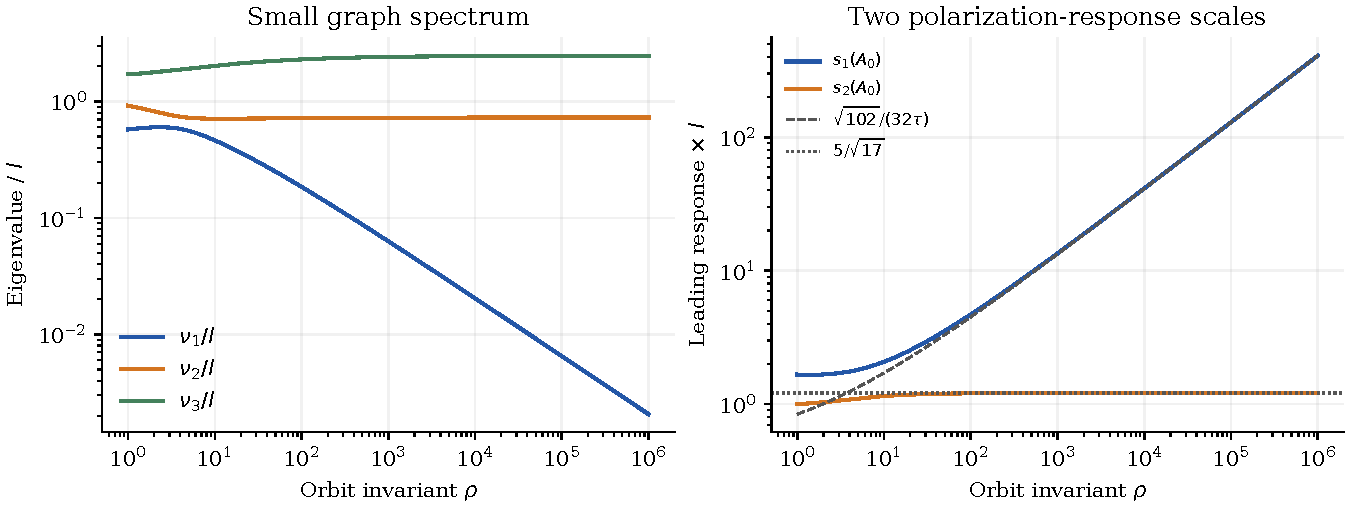
\includegraphics[width=\textwidth]{figures/output/fig02_finite_scales.pdf}
\caption{Finite models along $k/l=3/5$. Left: the three graph eigenvalues
 divided by $l$ for the weights in \eqref{eq:weak-weights}. Right: the two
 singular values of $A_0(\tau)$, equal to $l$ times the leading
 polarization-response singular values. Here $\rho$ and $\tau$ are related
 by \eqref{eq:tau-relation}. The dashed and dotted lines are the proved leading
 constants in \eqref{eq:finite-two-scales}. These are finite-model
 calculations, not numerical solutions of the HE equation.}
\label{fig:finite-scales}
\end{figure}

The additional weak scale is therefore visible both in the graph spectrum
and in one direction of the intrinsic metric derivative. The other
polarization direction retains scale $l^{-1}$, as the exact identity in
\eqref{eq:response-directions} explains.

\FloatBarrier
\begin{thebibliography}{Wue26c}

\bibitem[CT24]{clarketipler2024}
A.~Clarke and C.~Tipler,
\emph{Semi-stability and local wall-crossing for Hermitian Yang--Mills connections},
J. Symplectic Geom. \textbf{22} (2024), no.~3, 673--694.
Theorem and proposition locators refer to
\href{https://arxiv.org/abs/2304.05245v1}{arXiv:2304.05245v1}.

\bibitem[Del25]{delloque2025}
R.~Delloque, \emph{Continuity of HYM connections with respect to metric variations},
J. London Math. Soc. (2) \textbf{112} (2025), no.~1, e70219.
\href{https://doi.org/10.1112/jlms.70219}{doi:10.1112/jlms.70219}.
Locators refer to the published-version text
\href{https://arxiv.org/abs/2403.16814v4}{arXiv:2403.16814v4}.

\bibitem[Kob87]{kobayashi1987}
S.~Kobayashi, \emph{Differential Geometry of Complex Vector Bundles},
Publications of the Mathematical Society of Japan, vol.~15,
Princeton University Press, Princeton, NJ, 1987.
\href{https://www.mathsoc.jp/assets/pdf/publications/pubmsj/Vol15.pdf}{Mathematical Society of Japan edition}.

\bibitem[Stacks]{stacks}
The Stacks Project Authors, \emph{The Stacks Project},
\href{https://stacks.math.columbia.edu/tag/01XT}{Tag 01XT (cohomology of projective space)}
and \href{https://stacks.math.columbia.edu/tag/0BED}{Tag 0BED (K\"unneth formula)},
accessed October 31, 2026.

\bibitem[Wue26a]{wuebben2026response}
B.~J.~Wuebben, \emph{Metric response and Hermitian Yang--Mills flow
for two-step extensions}, preprint, October 27, 2026.
\href{https://doi.org/10.5281/zenodo.23717742}{doi:10.5281/zenodo.23717742}.

\bibitem[Wue26b]{wuebben2026bipartite}
B.~J.~Wuebben, \emph{Uniform Hermitian--Einstein spectra for bipartite
two-step extensions}, preprint, October 27, 2026.
\href{https://doi.org/10.5281/zenodo.23717660}{doi:10.5281/zenodo.23717660}.

\bibitem[Wue26c]{wuebben2026repeated}
B.~J.~Wuebben, \emph{Uniform Hermitian--Einstein spectra with repeated
stable factors}, preprint, October 29, 2026.
\href{https://doi.org/10.5281/zenodo.23780241}{doi:10.5281/zenodo.23780241}.

\end{thebibliography}

\end{document}
